% !TeX encoding = UTF-8

%==============================================================================
% Modelo de Dissertação para Trabalho de Conclusão de Curso Ciência da Computação
% do Centro Universitário Dinâmica das Cataratas de Foz do Iguaçu
% Autor: Miguel Diogenes Matrakas, Thiago Medeiros de Souza
% 2016/2017
% ---
%
% ADAPTADO DE:
% Modelo de Tese/Dissertação
% Autora: Fabiana Frata Furlan Peres 
% 2014 
% ---
%
% ADAPTADO DE:
% modelo de Documento TCC da Unioeste   
% que por sua vez foi ADAPTADO DE: 
% abtex2-modelo-trabalho-academico.tex, v-1.6 laurocesar
% Copyright 2012-2013 by abnTeX2 group at http://abntex2.googlecode.com/ 
% ---
% abnTeX2: Modelo de Trabalho Academico (tese de doutorado, dissertacao de
% mestrado e trabalhos monograficos em geral) em conformidade com 
% ABNT NBR 14724:2011: 
% Informacao e documentacao - Trabalhos academicos - Apresentacao
%==============================================================================

%==============================================================================
% DECLARAÇÃO DO TIPO DE DOCUMENTO, TAMANHO DA FOLHA E FONTE
%==============================================================================
\documentclass[12pt,oneside,a4paper,english,brazil]{cc-udc-abntex2}


%==============================================================================
% DEFINIÇÃO DOS PACOTES UTILIZADOS
%==============================================================================
\usepackage{cmap}		% Mapear caracteres especiais no PDF
%\usepackage{lmodern}	% Usa a fonte Latin Modern			
%\usepackage{uarial}		% Usa a fonte uarial - um clone livre da fonte arial (arial é uma fonte comercial, protegida)
%\usepackage{helvet}
\usepackage[T1]{fontenc}% Selecao de codigos de fonte.
\usepackage[utf8]{inputenc}	% Codificacao do documento (conversão automática dos acentos)
\usepackage{indentfirst}% Indenta o primeiro parágrafo de cada seção.
%\usepackage{color}		% Controle das cores
\usepackage{graphicx}	% Inclusão de gráficos
\usepackage{amsmath}	% Definições da Sociedade Americana de Matemática
\usepackage{amssymb}	% Definições da Sociedade Americana de Matemática
\usepackage{amsthm}		% Definições da Sociedade Americana de Matemática
\usepackage{hyphenat}	% comandos para separação silábica
\usepackage[alf,abnt-emphasize=bf,bibjustif]{abntex2cite} % Citações padrão ABNT
%\usepackage{pifont}		% Fonte de simbolos matemáticos
%\usepackage{latexsym}	% Fonte de simbolos
%\usepackage{url}		% Formatação de URLs - quebra de linha nas referências
%\usepackage{multirow}	% Celulas de tabela que ocupam multiplas linhas
%\usepackage{longtable}	% Tabelas longas, em mais de uma página
%\usepackage{marginnote} % Anotações nas margens do documento
%\usepackage[listofformat=subparens,subrefformat=parens,labelformat=parens]{subfig}		% utilização de subfiguras
%==============================================================================
% Pacotes de desenho - criar gráficos, plotar equações, anotar figuras, etc
\usepackage{tikz}		% Ferramenta principal
\usepackage{pgfplots}	% Desenhar gráficos no latex
\usetikzlibrary{positioning}
\usetikzlibrary{calc}
\usetikzlibrary{arrows,shapes,backgrounds}
\pgfplotsset{compat=newest}
%==============================================================================

%==============================================================================
% Caminhos para os diretório com as Imagens
%==============================================================================
\graphicspath{{./Imagens/}{./Graficos/}}

%==============================================================================
% Informações a respeito do trabalho
%==============================================================================
% ---
% INFORMAÇÕES REFERENTE A DISSERTAÇÃO
% ---

\titulo{Estudo e Implementação de um Sistema de Reconhecimento de Faces em Vídeo com o Algoritmo \textit{EigenFaces} na linguagem JAVA}
\autor{Thiago Correa Lima Da Silva}
\autorcitado{SILVA, Thiago da}
%\segundoautor{Andreia Matheus Cavalho}
%\segundoautorcitado{Carvalho, Andreia Matheus}
\orientador{Prof. Ma. Alessandra Bussador}
%\coorientador{Prof. Esp. Nome do Coorientador}
\data{2018}
\codigoautor{S586e} % solicitar o código ao bibliotecário da instituição
\codigopublicacao{ CDU: 004 }  % solicitar o código ao bibliotecário da instituição - Também pode ser padrão -> CDU: 02:141:005.7
\palavrachaveum{Reconhecimento de Faces em Vídeo}
\palavrachavedois{EigenFaces}
\palavrachavetres{OpenCV}
\palavrachavetres{JavaCV}
\palavrachavetres{JAVA}
\palavrachavetres{PCA - Principal Component Analisys}
\palavrachavetres{ACP - Análise de Componentes Principais}
 % DADOS para CAPA e FOLHA DE ROSTO


%==============================================================================
% CONFIGURAÇÕES DA APARENCIA DO PDF FINAL
%==============================================================================
\makeatletter
\hypersetup{     	
	pdftitle={\@title}, 
	pdfauthor={\@author},
	pdfsubject={\imprimirpreambulo},
	pdfcreator={LaTeX with abnTeX2},
	pdfkeywords={}{}{}{}, 
	colorlinks=true,       		% false: boxed links; true: colored links
	linkcolor=black,          	% color of internal links
	citecolor=black,        	% color of links to bibliography
	filecolor=black,      		% color of file links
	urlcolor=black,
	bookmarksdepth=3
}
\makeatother
 


%==============================================================================
% Constroi o índice remissivo
%==============================================================================
\makeindex


%==============================================================================
% SEPARAÇÃO DE SILABAS
% Incluir palavras que o LaTeX não realizar a separação silábica corretamente no texto
%==============================================================================
%\hyphenation{}
\hyphenation{Mar-ca-ção}
\hyphenation{lin-gua-gem}
\hyphenation{pro-fis-sio-nais}
\hyphenation{ar-qui-vos}
\hyphenation{fer-ra-men-tas}
\hyphenation{ma-te-ri-al}


%-----------------------------
%% para code listing
\usepackage{listings}
\usepackage{color}

\definecolor{dkgreen}{rgb}{0,0.6,0}
\definecolor{gray}{rgb}{0.5,0.5,0.5}
\definecolor{mauve}{rgb}{0.58,0,0.82}

\lstset{frame=tb,
	language=Java,
	aboveskip=3mm,
	belowskip=3mm,
	showstringspaces=false,
	columns=flexible,
	basicstyle={\small\ttfamily},
	numbers=none,
	numberstyle=\tiny\color{gray},
	keywordstyle=\color{blue},
	commentstyle=\color{dkgreen},
	stringstyle=\color{mauve},
	breaklines=true,
	breakatwhitespace=true,
	tabsize=3
}

%----------------------

%==============================================================================
% INÍCIO DO DOCUMENTO
%==============================================================================
\begin{document}
\frenchspacing % Retira espaço extra obsoleto entre as frases.

%==============================================================================
% ELEMENTOS PRÉ-TEXTUAIS
%==============================================================================
\imprimircapa
\imprimirfolhaderosto* % (o * indica que haverá a ficha bibliográfica)

%\input{Configuracoes/ficha_catalografica}
%\imprimirfichacatalografica

%% ---
% FOLHA DE APROVAÇÃO
% ---
\begin{folhadeaprovacao}
\begin{center}
	\vspace*{1cm}  
  	\large\textbf{TERMO DE APROVAÇÃO}
  	
  	\vspace*{1cm}
  	%\vspace*{2cm}
  	{\large\textbf\imprimirautor}

   \vspace*{1cm}
   %\vspace*{2cm}
    {\large\textbf\imprimirtitulo}   
 \end{center}     
  
	
	\hspace{.4\textwidth}
	\SingleSpace\noindent\normalsize{Trabalho de conclusão de curso apresentado como requisito obrigatório para obtenção do título de Bacharel em Ciência da Computação do Centro Dinâmica das Cataratas - UDC, Foz do Iguaçu, pela seguinte banca examinadora:}
%	\noindent\paragraphq
   
 %  \end{center}
    
   %\vspace*{1.5cm}
   \vspace*{0.5cm}  %minha modif
   \assinatura{{\imprimirorientador}\\{\small \imprimirinstituicao\\(Orientador)}}
   \assinatura{Prof. Banca 2\\{\small\imprimirinstituicao}}
   \assinatura{Prof. Banca 3\\{\small\imprimirinstituicao}}
   \vspace*{2.5cm}
   \begin{center}
   	{\imprimirlocal, \ \imprimirdata}
   	%{Foz do Iguaçu, 12 de junho de 2016}
   \end{center}
   
 
\end{folhadeaprovacao}
%% ---
% DEDICATÓRIA
% ---
\begin{dedicatoria}
   \vspace*{\fill}
   \begin{flushright}
   	\textit{Dedico este trabalho a meus pais, \\ Sr... e Sra... \\ que, com muito amor, me ensinaram os valores da vida.}
   	
   \end{flushright}
\end{dedicatoria}

%% ---
% AGRADECIMENTOS
% ---
\begin{agradecimentos}[AGRADECIMENTOS]

Agradeço a tudo e a todos, especialmente ao meu superior que incentivou e possibilitou o desenvolvimendo deste projeto em ambiente de trabalho, e à minha orientadora que,

\end{agradecimentos}


%% ---
% EPÍGRAFE
% ---
\begin{epigrafe}
    \vspace*{\fill}
	\begin{flushright}
		\textit{
		``Emancipate yourself from mental slavery,\\
		 none but ourselves can free our mind.''\\
		\-- Robert Nesta Marley (1979)	
		}
	\end{flushright}
\end{epigrafe}


%\vspace*{-0.65cm}
%% ---
% RESUMO PORTUGUÊS
% ---
\begin{resumo}[RESUMO]	
A rede social ....



 \vspace{\onelineskip}
    
 \noindent
 \textbf{Palavras-chaves}: Dados. Data Mining. Twitter. Python.
 % 4 palavras separadas por . (ponto)
\end{resumo}

%\vspace*{-0.65cm}
%% ---
% RESUMO INGLÊS
% ---
\begin{resumo}[ABSTRACT]
 \begin{otherlanguage*}{english}
The social network ....

   
   \vspace{\onelineskip}
 
   \noindent 
   \textbf{Keywords}: Data. Data Mining. Twitter. Python.
 \end{otherlanguage*}
\end{resumo}


%\pdfbookmark[0]{\listfigurename}{lof}		% inserir lista de ilustrações
%\listoffigures*
%\cleardoublepage

%\pdfbookmark[0]{\listtablename}{lot}			% inserir lista de tabelas
%\listoftables*
%\cleardoublepage

%\pdfbookmark[0]{\lstlistlistingname}{lol}	% inserir lista de códigos
%\counterwithout{lstlisting}{chapter}
%\begin{KeepFromToc}
%\lstlistoflistings
%\end{KeepFromToc}
%\cleardoublepage

%\pdfbookmark[0]{\listofgraficosname}{logr}	% inserir lista de gráficos
%\listofgraficos*
%\cleardoublepage

%% ---
% SIGLAS
% ---
\begin{siglas}
	\item[ACP] Análise de Componentes Principais
	\item[BMP] \textit{Windows Bitmap}
	\item[CDDL] \textit{Commun Development and Distribution License} - Licensa Comum de Desenvolvimento e Distribuição \footnotemark[1]	
	\item[FBI] \textit{Federal Bureal of Investigation} - Agência Federal de Investigação Americana \footnotemark[1]
	\item[FPS] \textit{Frames Per Second} - Quadros por Segundo \footnotemark[1]	
	\item[GNU/GPL] \textit{General Public License} - Licensa Pública Geral\footnotemark[1]	
	\item[GUI] \textit{Graphics User Interface} - Interface Gráfica para Usuário \footnotemark[1]		
	\item[IDE] \textit{Integrated Development Environment} - Ambiente Integrado de Desenvolvimento \footnotemark[1]	
	\item[JPG] \textit{Joint Photographic Experts Group}
	\item[NSA] \textit{National Security Agency} - Agência Nacional de Segurança \footnotemark[1]	
	\item[PDI] Processamento de Imagens
	\item[PCA] \textit{Principal Component Analisys} - Análise de Componentes Principais
	\item[PIXELS] \textit{Picture Elements} 
	\item[PNG] \textit{Portable Network Graphics} - Gráficos Portáteis para Rede \footnotemark[1]	
	\item[RGB] \textit{Red Blue Green}
	\item[UML] \textit{Unified Modeling Language} - Linguagem de Modelagem Unificada \footnotemark[1]	
	\item[XP] \textit{eXtreme Programming}
\end{siglas}

  				% inserir lista de abreviaturas e siglas

%\begin{simbolos}
  \item[$ \Gamma $] Letra grega Gama
  \item[$ \Lambda $] Lambda
  \item[$ \zeta $] Letra grega minúscula zeta
  \item[$ \in $] Pertence
\end{simbolos}
				% inserir lista de símbolos

\vspace*{0cm}
\pdfbookmark[0]{\contentsname}{toc}			% inserir o sumario
\tableofcontents*
\cleardoublepage


%==============================================================================
% ELEMENTOS TEXTUAIS
%==============================================================================
\textual
\pagestyle{abnt_CC-UDC}

% !TeX encoding = UTF-8

\chapter{INTRODUÇÃO}\label{ch:introducao}

O reconhecimento de face é um dos campos de pesquisa mais interessantes e importantes nas últimas duas décadas \cite{wei_lun}. Grandes empresas estão na corrida para ver quem desenvolve o melhor algoritmo de reconhecimento de faces, e apenas à pouco tempo, duas delas (Google e Baidu) conseguiram taxas de erros abaixo das apresentadas por seres humanos (que se acerca aos 8\%) \cite{stats_economy_compass_2017}.
 
As possibilidades de uso de um sistema de reconhecimento de faces são vastas (desde o uso comercial como empresas que querem identificar seus clientes e oferecer um serviço personalizado ao uso da polícia para o combate criminal e forense). Chega a ser um assunto polêmico em alguns círculos pois podem inferir em invasão de privacidade e privação da liberdade como a conhecemos.

As pesquisas sobre o assunto envolvem conhecimentos de disciplinas como neurociência, psicologia, computação visual, reconhecimento de padrões, processamento de imagens, matemática avançada \cite{wei_lun}, por isso apresenta um grande problema computacional. Além do problema de manipulação de imagens,  de identificação e reconhecimento das faces, deve-se considerar problemas de persistência destas, a questão de treinamento das faces, velocidade de verificação, de extração de dados de imagens e vídeos e desempenho em geral.


\section{Breve História}\label{sec:historia}

O reconhecimento automático de faces é um conceito relativamente novo. Desenvolvido na década de 60, o primeiro sistema semi-automático requeria que um administrador do sistema localizasse pontos da imagem como olhos, boca, nariz,  etc, e depois um algoritmos comparava as distâncias entre estes pontos em diferentes fotos para dar um resultado de comparação \cite{nstc_homeland}. Nos anos 80, algoritmos simples foram criados para automatizar este processo. Em 1988, Kirby e Sirovich aplicaram Análise de Componente Principal, uma técnica padrão de álgebra linear, para o problema de reconhecimento de face. Este foi considerado um marco pois mostrou que menos que 100 valores são requeridos para codificar uma imagem de uma face normalizada e bem posicionada \cite{nstc_homeland}. Em 1991, Turk e Pentland descobriu o erro residual das comparações feitas com a técnica \textit{eigenfaces} poderiam ser usadas para detectar faces em uma imagem - uma descoberta que permitiu detecção em tempo-real. Apesar desta abordagem ser imitado a posição da face, qualidade da imagem e fatores de ambiente, ela criou um significante interesse no desenvolvimento de tecnologias automáticas para reconhecimento \cite{nstc_homeland}. A tecnologia capturou a atenção da mídia e do público em janeiro de 2001 no evento \textit{SuperBowl}, que capturou rostos das imagens das câmeras de vigilância e comparou com fotos digitais "3x4" de uma base de dados apresentando rostos similares \cite{nstc_homeland}.

Hoje, o reconhecimento de faces está sendo usado no combate à fraude de passaportes e cédulas de identidades onde a foto é padronizada com ambiente controlado, aplicativos de celulares e redes sociais para entretenimento, enquanto que grandes governos e organizações patrocinam, incentivam e desafiam empresas para conseguir o algoritmo ideal de reconhecimento \cite{nyu_ccpr_frt}.



\section{Problemática}\label{sec:problematica}

A face é um objeto 3D iluminado por de fontes de luz e envolvida por um fundo (\textit{background}) com “dados arbitrários” (inclusive outras faces). Portanto, a aparência que uma face possui quando projetada para um modelo 2D pode variar tremendamente. Na verdade, problemas de iluminação e de segmentação “\textit{foreground-background}” tem sido questões pertinentes no campo da computação gráfica e visual como um todo \cite{tony_columbia}. Sendo assim o primeiro problema a enfrentar para o reconhecimento de faces seria a aquisição e processamento da imagem para que se possa detectar a face. As seções seguinte irão descrever procedimentos com mais detalhes. 


\subsection{Detecção e Aquisição da Face}\label{subsec:aquisicao_imagem}

Em geral, em uma imagem retirada de vídeo um digital de nível amador, o módulo de identificação da face deve encontrar condições luminosas descontroladas, alta variação de poses, maquiagem, mudanças nos pelos faciais, adoecimento, envelhecimento, oclusões da face por interferência, roupa ou cabelo, enfim, uma incontável gama de variáveis \cite{tony_columbia}. De fato, há diversos desafios e fatores chaves que podem significantemente impactar a performance da identificação e reconhecimento da face e os pontos de verificação (\textit{matching scores}).

Na \autoref{ex_variacao_fig}, lista-se exemplos de alguns destes desafios em imagens, respectivamente:

\begin{figure}[h]
	\centering
	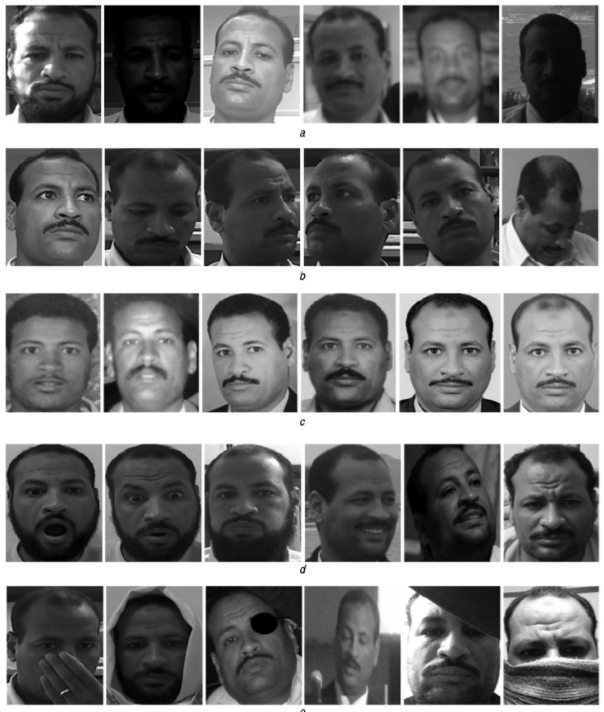
\includegraphics[width=.8\textwidth]{ex_variacao}
	\caption{Exemplos de Variação}
	\fonte{\textit{The Reseachgate.net}}
	\label{ex_variacao_fig}
\end{figure}


\begin{enumerate}[label=(\alph*)]
	\item Variação de iluminação;
	\item Variação de poses ou pontos de visão;
	\item Envelhecimento;
	\item Expressões faciais e estilo da face (pelos faciais ou maquiagem);
	\item Oclusão.
\end{enumerate}


A detecção contínua de faces em vídeos (diz-se \textit{tracking} ou rastreamento) segue a mesma lógica e tem os mesmo problemas de aquisições de faces estáticas. O rastreamento nada mais é do que a detecção contínua da face em \textit{frames} advindos de um vídeo, com um forte problema adicional de que deve-se manter a usabilidade do sistema em um computador contemporâneo de baixa a média performance. Em outras palavras, o processamento envolvido deve ser eficiente o bastante considerando o tempo de execução do vídeo (\textit{frames} por segundo) e do sistema e tempo de armazenamento e consulta de dados.

A performance da detecção da face é uma questão-chave no processo de reconhecimento, porém considerada bem para poses de faces frontais, deste a década de 90. A detecção de faces pode ser considerada um caso específico da área de detecção de objetos, alcançando confiáveis \cite{stats_face_detection_IEEE}.

Em um trabalho feito em 2003 por \cite{final_project_stanford} na Universidade de Stanford - Califórnia, utilizaram a técnica \textit{EigenFaces} para detecção, acrescido de algoritmo de identificação de gênero de sexo, com um \textit{Pentium 3} de 700 Mhz e menos de 500 megas de memória, alcançaram resultados que superam 93\% de taxa de sucesso nas condições mais adversas, considerando iluminação e escala (numero grande de faces em uma imagem). Outros \textit{benchmarks} mais recentes (2015) apresentam resultados que superam os 97.2\% \cite{stats_hong_kong}.

O problema com estas técnicas relativamente antigas, é que também reconhecem fotos de fotos, ou desenhos de faces como legítimas faces, por vezes até com pontuação bastante para uma verificação de sucesso com uma face real. Outro problema é estas técnicas não funcionam num angulo de perfil, ou de qualquer outro ângulo que não seja o frontal.

Novas técnicas de detecção não-frontais estão sendo implementadas, bem como as de modelagem sub-espacial 3D e comparações com reconhecimento de padrões baseados em aprendizado de máquinas e redes neurais, são fundamentos para os sistemas de reconhecimento de face avançados, capazes de reconhecer não só a face, mas também a estrutura cranial do alvo \cite{3dmodel_fd}. 

Após a face ser identificada e localizada na imagem, para que sirva ao processo de reconhecimento, deve-se recortar esta face da imagem e performar algumas operações gráficas sobre a mesma. Nesta fase são consideradas atividades de corte da face na região localizada, escalamento e correção de rotação, transformar em preto e branco, normalizar a imagem para minimizar as condições de ambiente da foto, deixando a face pronta para a próxima faze do processo: o treinamento.


\subsection{Treinamento e Reconhecimento da Face} \label{subsec:treinrecface}

Esta fase consiste em manipular a face recortada da imagem ou \textit{frame}, normalizada e tratada de forma a extrair informações e características desta para que se possa salvar de alguma forma e relacionar estas características com a pessoa ou alvo. Nesta fase é importante aquisitar fotos da mesma face mostrando diferentes expressões faciais e situações de lumiosidade e posição.

A forma que isso pode ser feito depende totalmente do algoritmo de reconhecimento envolvido. Há várias técnicas e algoritmos de reconhecimento, como \cite{issues_methods_FR}:

\begin{itemize}
	\item reconhecimento baseado em redes neurais;
	\item reconhecimento baseado em processamento 3D;
	\item reconhecimento baseado em descritores de face;
	\item reconhecimento baseado em reconstrução;
	\item reconhecimentos tradicionais ou clássicos, dentre outros;
\end{itemize}

Este trabalho se focará em dois dos algoritmos clássicos, famosos por serem pioneiros e objetos de muito estudo, testes e documentação: \textit{EigenFaces} e \textit{FisherFaces}. Os algoritmos convencionais podem ser divididos em duas categorias: caracterização holística ou linear, sendo que \textit{EngenFaces} e \textit{FisherFaces} fazem parte da primeira, que fazem parte de outra subdivisão de métodos de projeção linear chamada Análise de Componentes Principais - ACP (ou no inglês, \textit{Principal Component Analysis} – PCA) \cite{issues_methods_FR}.

Basicamente, o método ACP consiste em tratar a imagem de uma forma uniforme, coletar características da mesma transformando-as em valores numéricos e disponibilizá-las em um plano cartesiano, que pode ter mais de três dimensões. Este processo visa destacar discrepâncias da face, ou seja, padrões de mudança de constaste, de relevo ou sombreamentos, ou diferença de cores. A transformação destes valores manipulados de volta em imagens, cria os chamados \textit{EngenFaces} (Faces de fantasmas, em Alemão), pois como mostra a \autoref{someeigen}, é devido a sua estranha aparência \cite{drmathew_java_programming}.

\begin{figure}[h]
	\centering
	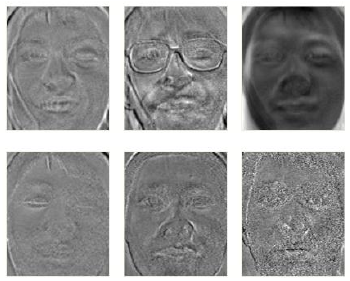
\includegraphics[width=.6\textwidth]{someeigen}
	\caption{Exemplos de EigenFaces}
	\fonte{\cite{drmathew_java_programming}}
	\label{someeigen}
\end{figure}

O objetivo é que uma imagem de treinamento possa ser decomposta em uma soma múltiplas \textit{eigenfaces} medidas e disponibilizadas em uma sequencia especial.

Uma maneira mais simples de representar o relacionamento entre \textit{eigenfaces} e imagens das faces é quem estas faces são disponibilizadas em um espaço multidimensional, ou um plano cartesiano "\textit{n}" dimensões onde os eixos do plano são as \textit{eigenfaces} \cite{drmathew_java_programming} como ilustra a  \autoref{eigencartesiano}.

Tendo a face (ou faces) relacionada com o alvo, representado em valores e disponibilizada em um plano cartesiano de “n” dimensões, resta a verificação ou reconhecimento da face contra outra. 

Para o reconhecimento da face propriamente dito, o mesmo processo do treinamento deve ser repetido e a face representada e disponibilizada no mesmo plano cartesiano das faces treinadas \cite{drmathew_java_programming}. A distância entre as duas faces representadas no plano cartesiano é medida, e basicamente, quando menor a distância, maior é a taxa de reconhecimento. Ou seja, uma distância zero entre as duas faces representadas no plano seria uma correspondência perfeita. A \autoref{eigencartesiano} abaixo ilustra esta descrição:

\begin{figure}[h]
	\centering
	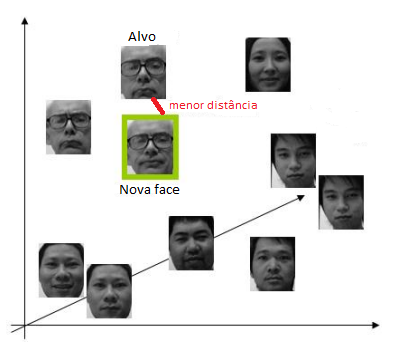
\includegraphics[width=.6\textwidth]{eigencartesiano}
	\caption{Exemplos de EigenFaces}
	\fonte{Adaptado de \cite{drmathew_java_programming}}
	\label{eigencartesiano}
\end{figure}

Este plano cartesiano, na prática, pode ser um arquivo binário ou texto, comumente chamado de "\textit{bundle}".

\section{OBJETIVOS}\label{sec:objetivos}
Este projeto propõe a implementação de um Sistema de Reconhecimento de Faces em Vídeo utilizando dois algoritmos desenvolvidos para este fim: \textit{FisherFaces} e \textit{EigenFaces}.

O algoritmo \textit{EigenFaces} será implementado seguindo as instruções e exemplos de código de \cite{drmathew_java_programming}. Quanto ao algoritmo \textit{FishFaces}, será usado a implementação da biblioteca OpenCV. Haverá uma tentativa de fazer com que os dois algoritmos funcionem juntos para que se use os pontos fortes de cada um para melhorar a taxa de reconhecimento. 

\subsection{Objetivos Específicos}\label{sec:organizacao-trabalho}

O desenvolvimento do sistema se fará na exploração das seguintes fases:

\begin{itemize}
	\item Análise das bibliotecas e suas versões para melhor escolha;
	\item Preparação do ambiente;
	\item Implementação da interace e manipulação de imagens (e vídeos)  utilizando componentes Java e as bibliotecas gráficas (para  recorte de frames e imagens, aplicação de filtros, mineração de dados da imagem, manipulação de cores, iluminação, normalização, etc);
	\item Implementação do algoritmo EigenFaces;
	\item Detecção de face em imagens tiradas com câmera;
	\item Treinamento / reconhecimento de face na imagem;
	\item Incrementar a implementação feita acima para o treinamento  e reconhecimento em vídeo tirado da câmera em tempo real;
	\item Integrar os algoritmos de outras implementações;
	\item Performar uma bateria de testes, e comparar resultados.
\end{itemize}

O objetivo final é criar um sistema de reconhecimento de faces em vídeo, analisando seus resultados e finalmente disponibilizando todo o trabalho e o código aberto ao público desenvolvedor e acadêmico.


\section{Justificativa} 

O reconhecimento de faces é umas das tecnologias mais estudadas e complexas de hoje em dia. As maiores empresas e governos do planeta estão na corrida para se acercarem aos 100\% de acerto em seus reconhecimentos e governos e organizações como FBI e NSA investem e desafiam os produtores desta tecnologia \cite{nstc_homeland}.

Eis na \autoref{tabelaempresasrecog} algumas das empresas quem produzem tecnologias de reconhecimento de ponta:

\vspace*{5cm}
\begin{table}[h]
	\centering
	\caption{Empresas que produzem tecnologias de reconhecimento de faces}
	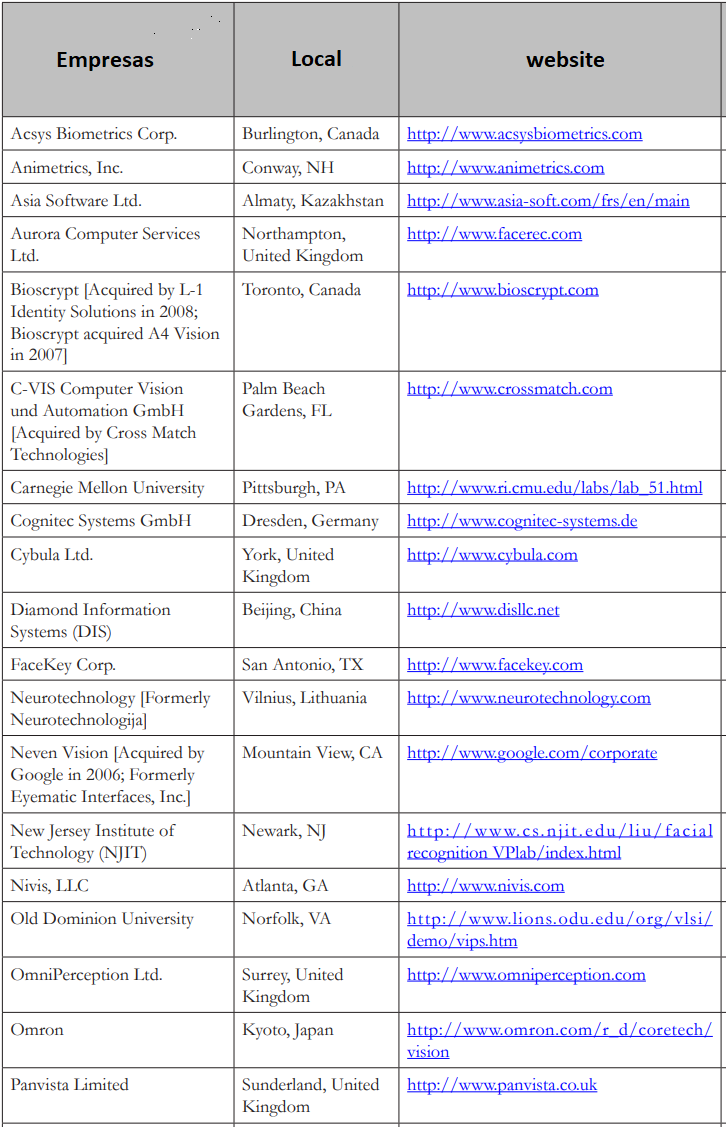
\includegraphics[width=.6\textwidth]{tabelaEmpresasRecog}
	\fonte{Adaptado de \cite{nstc_homeland}}
	\label{tabelaempresasrecog}
\end{table}



As pioneiras estão avançando exponencialmente no assuntos e empresas a Google e a Baidu já conseguem taxas de erros menores do que as alcançadas por seres humanos, com rapidez de verificação sem precedentes, como mostra a \autoref{statstoprecog}.

\vspace*{10cm}
\begin{figure}[h]
	\centering
	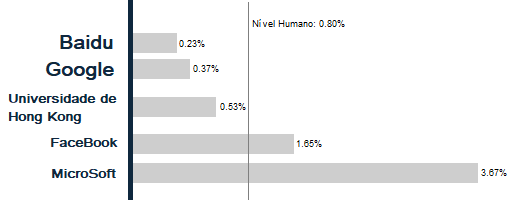
\includegraphics[width=.9\textwidth]{stats_toprecog}
	\caption{Comparação de sistemas de reconhecimento de faces em percentagem (\%) de erros}
	\fonte{Adaptado de \cite{stats_economy_compass_2017}}
	\label{statstoprecog}
\end{figure}


A \autoref{statstoprecog} mostra que a tecnologia da empresa chinesa Baidu está liderando a corrida com apenas 0.23\% de taxa de erro, contra 0.37\% da empresa americana Google \cite{stats_economy_compass_2017}. Ambas já conseguiram ultrapassar as taxas alcançadas por seres humanos, que como mostra a \autoref{statstoprecog}, atinge a taxa de 0.8\% de erros. Como mostra \cite{stats_economy_compass_2017}, os humanos em geral não são uma fonte 100\% precisa para reconhecimento de faces. Humanos podem facilmente confundir pessoas, ou não reconhecê-las pela idade ou por mudança de aparência ou estilo, ou até esquecê-las.

No final de 2016, a Baidu implantou seu sistema em sua histórica “Cidade de Água”, substituindo totalmente o sistema de cartões e \textit{tickets} com 99\% de sucesso \cite{baidiu_theverge}, e já estão no processo de implantação em outros parques temáticos. Policiais chineses estão usando óculos de reconhecimento que verificam instantaneamente as faces de turistas e procurados. Com os armazenamentos e reconhecimentos dominando aplicativos de celulares e redes sociais, e a polícia com grande interesse forense no assunto, e outras infinitas possibilidades, obviamente esta tecnologia fará parte do dia a dia do nosso futuro, sendo assim é necessário estuda-la, entendê-la e desenvolvê-la.












%==============================================================================
% CAPÍTULOS DA DISSERTAÇÃO
%==============================================================================
% !TeX encoding = UTF-8

\chapter{REVISÃO BIBLIOGRÁFICA}\label{ch:rev-bibs}

Vários trabalhos serviram como fonte de conhecimento e suporte para o entendimento e desenvolvimento deste tema. Alguns foram considerados mais importantes por abordar detalhadamente o problema de reconhecimento, outros foram buscados para se entender melhor, ou ter outra visão sobre alguns detalhes específicos do problema.

Trabalhos de autores como \cite{geysilva} ajudaram a estruturar e organizar o tema por abordar tópicos similares e por possuir riqueza de detalhes no assunto de análise de componentes apresentando uma implementação em \textit{MatLab} (um \textit{software} interativo voltado para o cálculo numérico).

O trabalho de \cite{img-digital-willians} foi utilizado para se aprofundar no tema de imagens digitais, assim como  \cite{gonzalez_woods} que também esclareceu o funcionamento de escalonamento, normalização e mono cromatização de imagens. O autor Dr. Andrew Davison em seu livro \cite{drmathew_java_programming} se destacou pela ótima didática facilitando o entendimento de Análise de Componentes e sua relação com \textit{EigenFaces}, disponibilizando ainda exemplos de implementação em \textit{JAVA}. 

Os trabalhos \cite{tutorial_en_smith} e \cite{tutorial_pt} foram estudados como tutoriais do processo de ACP e será usado posteriormente como guias de implementação do algoritmo.

Nas próximas seções serão explanados os conteúdos destes e de outros trabalhos disponibilizados em uma ordem didática.


\section{Conceitos de Aquisição e Processamento de Imagens}\label{sec:processamento_imagens}

Com a abrangência dos sistemas de comunicação, com difusão de conhecimentos informações pelos diversos meios, captar, armazenar e processar imagens se tornou necessidade fundamental. Para o reconhecimento de faces em vídeo, o sucesso deste processo é pré-requisito  para o funcionamento dos algoritmos. 

As sessões a seguir contemplam fundamentos básicos sobre imagem, vídeo, a alguns de seus processamentos necessários para a aplicação dos algoritmos de detecção e reconhecimento de faces.


\subsection{Imagem Digital}\label{subsec:imagem}

A imagem digital são valores numéricos disponibilizados em uma matriz bidimensional. Basicamente existem dois tipos de imagens: os chamados \textit{rasters} ou \textit{bitmaps}, e vetorizadas. A primeira são representações de cada ponto da imagem com alguma cor usadas geralmente em fotografias, enquanto que o segundo é produzido por plotadores que recebem os pontos e as distâncias entre eles como parâmetros, considerando retas, curvas, polígonos e etc, sendo assim não perdem sua qualidade quando redimensionados.

Converter uma imagem para o formato digital significa transferir os elementos que a compõem para elementos representativos de cada pequeno fragmento original. O menor elemento da imagem, o \textit{pixel}, é identificado segundo sua intensidade de nível de cinza e as cores correspondentes. Identificados, estes elementos são armazenados por códigos que podem ser reconhecidos pelo dispositivo de visualização e apresentados novamente por um dispositivo de visualização, como um monitor de vídeo ou impressora \cite{img-digital-willians}. 

%\vspace*{13cm}
\begin{figure}[h]
	\centering
	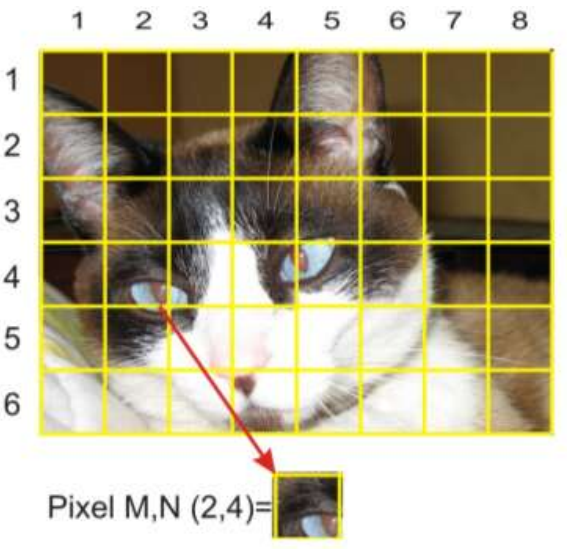
\includegraphics[width=.6\textwidth]{pixel-img}
	\caption{Exemplo de imagem representada como uma matriz (M,N) de pixels, com destaque para o pixel (2,4).}
	\fonte{\cite{img-digital-willians}}
	\label{pixel_img}
\end{figure}


Para que uma imagem analógica (representação real da cena) seja convertida, esta deve sofrer uma separação espacial (amostragem) e em amplitude (quantização) \cite{img-digital-willians}. 

A amostragem é a divisão do plano (x, y) em uma grade (ou matriz bi-dimensional) onde \textit{x} e \textit{y} serão números inteiros. Os pontos da matriz de são denominados \textit{pixels} (\textit{PICTure Elements}), como ilustra a \autoref{pixel_img}. Cada pixel representa uma parte da cena real, desta forma a resolução espacial da imagem é proporcional aos valores de M e N correspondentes na matriz (ao exemplo da \autoref{pixel_img}). Em geral a malha de amostragem, o formato dos pixels (x,y), é retangular, mas pode também ser triangular ou mais complexa. Os valores de cada ponto da matriz, coluna \textit{x} e linha \textit{y}, que identifica um único pixel (M,N), devem ser escolhidos de forma a respeitar a relação qualidade da imagem \textit{vs.} espaço de armazenamento, em função da aplicação para a qual a imagem se destina. Para uma imagem digital com 256 níveis de cinza o número de bytes ocupados para armazenar a imagem é o produto da linha com a coluna da matriz \cite{img-digital-willians}. 

Matematicamente, toda imagem monocromática (preto e branco) é um função $f(x,y)$ da intensidade luminosa, em qualquer parte das coordenadas (x,y), proporcional ao brilho (tons de cinza) da imagem em um determinado ponto. A \autoref{pixel_img}) mostra uma imagem e como representamos os eixos x e y no plano cartesiano \cite{gonzalez_woods}. 

A função  $f(x,y)$  é a multiplicação da iluminância  i(x,y) (que é a quantidade de luz que incide sobre o objeto) pela refletância  r(x,y)  (que é fração de luz incidente que o objeto vai refletir ao ponto (x,y). 

Sendo assim, podemos dizer que :

$f(x,y) = i(x,y) * r(x,y)$,

onde $0 < i(x,y)$ e $0 < r(x,y) < 1$ .

Quando se utiliza uma imagem colorida, no padrão RGB por exemplo,  deve se usar uma função $f(x,y)$ para cada banda, R(\textit{Red}), G(\textit{Green}) e B(\textit{Blue}) que são as cores primárias\cite{gonzalez_woods}.

 
\subsection{Formato PNG}\label{subsec:png}

O PNG (\textit{Portable Network Graphics} ou "\textit{PNG is Not Giff}") é um formato de representação de imagens do tipo \textit{rasters} e foi desenhado para substituir o formato GIF e o TIFF em certa extensão. O PNG tem 3 vantagens principais: suporta canal alfa (transparência) de forma eficiente, tem a maior gama de profundidade de cores e alta compressão que pode ser regulável. Além disso, o formato é livre enquanto os outros possuem patentes \cite{png}. 

O trabalho da compressão é justamente retirar essas informações redundantes para diminuir o peso do arquivo. Por exemplo, dado um pixel qualquer de uma imagem, possivelmente, a cor ou o valor desse pixel será igual a de vários outros elementos dentro da mesma imagem. Quando a imagem é comprimida, para excluir os pixels de valores iguais, é guardado apenas um valor desse pixel, que é reproduzido para os outros semelhantes, economizando tempo de carregamento \cite{img_compact}. Outras técnicas mais complexas também são utilizadas.

Este formato que ocupa pouco espaço em memória e de fácil manipulação foi escolhido neste trabalho para a representação de imagens digitais quando for necessário.

 \subsection{Vídeo Digital}\label{subsec:videodigi}
 
 Um vídeo é uma sucessão de imagens apresentadas sequêncialmente em um determinado ritmo. O olho humano pode distinguir cerca de 20 imagens por segundo. Deste modo, quando se mostram mais de 20 imagens por segundo, é possível enganar o olho e criar a ilusão de uma imagem em movimento. 
 
 A fluidez de um vídeo se caracteriza pelo número de imagens por segundo (frequência de quadros), expresso em FPS (Frames per second - Quadros por segundo). o vídeo multimídia é geralmente acompanhado de som, ou seja, dados de áudio \cite{ccm_video_digi}.

\subsection{Aquisição da Imagem e de Vídeo}\label{subsec:aquisicao_video}

No processo de aquisição de imagens, tradicionalmente, uma "cena" tridimensional (ou imagem analógica) deve ser capturada por um dispositivo eletrônico, que colhe uma amostragem convertendo-a para uma imagem digital de duas dimensões. Por exemplo, uma câmera digital captando uma cena 3D e convertêndo-a em 2D.

Atualmente o dispositivo de conversão mais usado  é a câmera CCD (\textit{charge coupled device}), que é uma matriz de células semi-condutoras fotossensíveis que trabalham com capacitadores, fazendo um armazenamento da carga elétrica proporcional à energia luminosa incidente \cite{gonzalez_woods}.

A saída deste processo é a imagem do tipo \textit{raster}, pronta pra ser formatada e compactada por alguma representação (PNG, JPG, BPM, etc). 


Na aquisição de vídeos, o mesmo processo descrito acima para imagens é utilizado, com a diferença de que o vídeo é uma fluidez de imagens, sendo assim é necessário aplicar este processo iterativamente. Caso uma única imagem precise ser colhida do vídeo, basta escolher um quadro (descrito na \autoref{subsec:videodigi}) para o processo.

\subsection{Processamento da Imagem}\label{subsec:processamento}

O processamento de imagem é todo o processo que tem uma imagem como entrada e saída, tais como fotografia ou quadros de vídeo \cite{inpe_proc_img}. 

Usa-se para melhorar o aspecto visual de certas feições estruturais para o analista humano ou para performance e para fornecer outros subsídios para a sua interpretação, inclusive gerando produtos que possam ser posteriormente submetidos a outros processamentos \cite{inpe_proc_img}.

O processamento de imagens pode ser dividido em 3 fases básicas: pré-processamento, realce e classificação.
Pré-processamento refere-se ao processamento inicial de dados brutos para calibração radiométrica da imagem, correção de distorções geométricas e remoção de ruído.
Realce visa melhorar a qualidade da imagem, permitindo uma melhor discriminação dos objetos presentes na imagem.
Na classificação são atribuídas classes aos objetos presentes na imagem \cite{inpe_proc_img}.

Nas próximas seções algumas técnicas de processamento de imagens serão abordadas pela sua importância e sua necessidade de uso em algoritmos de detecção e reconhecimento de faces. São elas:

\begin{itemize}
	\item Conversão em Escala de Cinza: considerada uma técnica pré-processamento, é usada para transformar a imagem em "preto e branco" (na escala de cinza) , o que torna outras operações de processamento mais rápidas e eficientes;
	\item Escalonamento: pré-processamento de correção linear geométrica 2D \cite{lapix_escala};
	\item Equalização: uma técnica de realce de contraste \cite{gonzalez_woods}
	\item Segmentação: recorte da imagem, onde se extraem os objetos relevantes para a aplicação desejada \cite{inpe_proc_img}.
	\item Classificação: uso de classificadores para reconhecer padrões em imagens \cite{drmathew_java_programming}
\end{itemize}

\subsubsection{Conversão em Escala de Cinza}\label{subsubsec:filtros}

Em fotografia, computação e colometria, uma imagem em escala de cinza é uma imagem em que cada valor de pixel é uma única amostra da representação de intensidade de luz \cite{stephen_greyscale}. Em outras palavras, o valor R, G e B de cada pixel devem ser iguais para se obter uma escala de cinza que varia de preto em sua intensidade mais baixa para o branco absoluto.

A conversão de uma cor para escala de cinza não é algo único. Existem diversas maneiras e possibilidades de inserção de parâmetros que dariam resultados diferentes. A maneira mais usual é calcular a média dos valores RGB de cada pixel e atribuir o resultado ao pixel novamente. Exemplo:

$ Gray = (Red + Green + Blue) / 3 $, reconhecendo que o algoritmo seria algo como:

\begin{lstlisting}
For Each Pixel in Image {
	Red = Pixel.Red
	Green = Pixel.Green
	Blue = Pixel.Blue
	Gray = (Red + Green + Blue) / 3	
	Pixel.Red = Gray
	Pixel.Green = Gray
	Pixel.Blue = Gray
}
\end{lstlisting}



Converter a imagem em escala de é necessário para tornar eficientes os subsequente processos, como equalização e aplicação de classificadores \cite{drmathew_java_programming}. Na \autoref{fig:escalacinza} apresenta-se um exemplo desta tipo de conversão.

\begin{figure}[h]
	\centering
	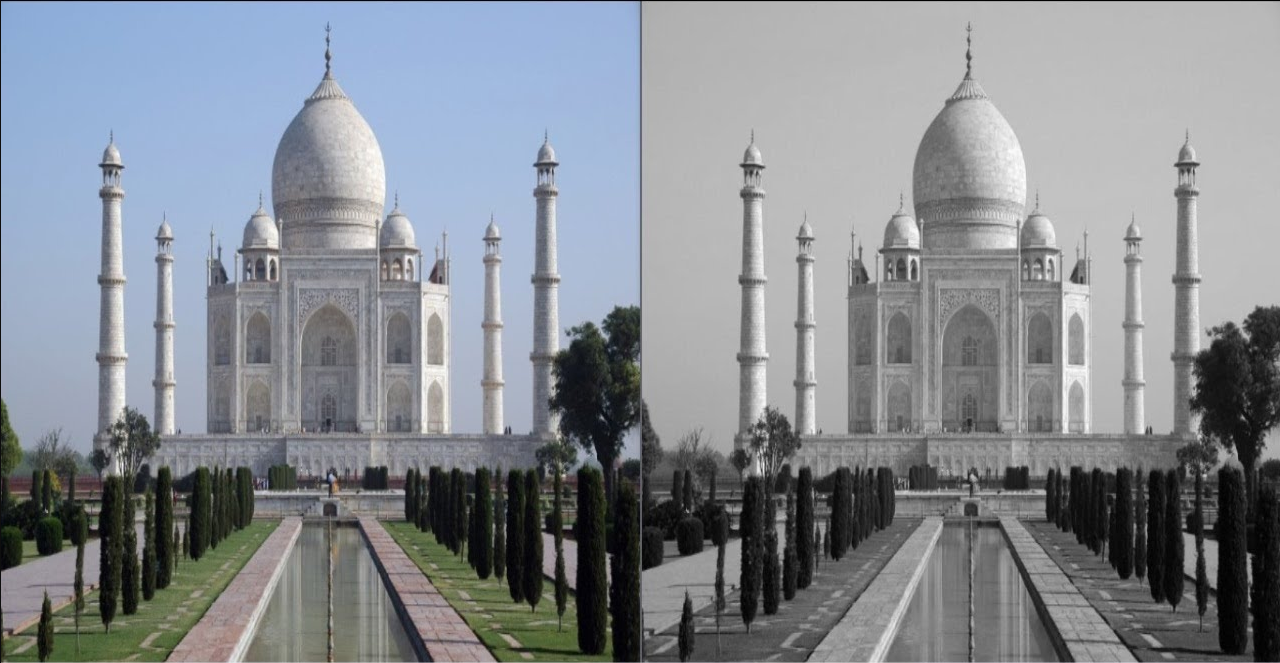
\includegraphics[width=.7\textwidth]{escalacinza}
	\caption{Imagem convertida para escalada de cinza.}
%	\fonte{\cite{lapix_escala}}
	\label{fig:escalacinza}
\end{figure}

\subsubsection{Escalonamento}\label{subsubsec:escalonamento}

O escalonamento de imagens é uma transformação geométrica 2D. Pontos no Plano $(x, y)$ podem ser escalonados (esticados) por fatores de escala, definida como $S_x$ e $S_y$, através de multiplicação \cite{lapix_escala}:

$ x’ = x . S_x $, $ y’ = y . S_y $.
Onde o novo ponto é resultado da multiplicação do ponto pela escala.

No exemplo da figura abaixo $S_x=2$ e $S_y=1$ os valores de $x$ foram escalonados em 2 ($ S_x $) enquanto y foi escalonado em 1 ($ S_y $). Observe o resultado a seguir.:

\begin{figure}[h]
	\centering
	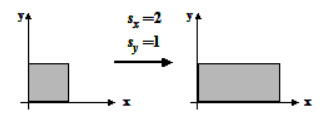
\includegraphics[width=.6\textwidth]{escala}
	\caption{Escalonamento com $S_x=2$ e $S_y=1$.}
	\fonte{\cite{lapix_escala}}
	\label{fig:escala}
\end{figure}

O escalonamento pode causar distorções na imagens se não for feita linearmente, e perda de qualidade caso os valores sejam alterados de forma a aumentar a imagem. É muito usado para padronização de tamanhos, e se o escalonamento for feito com a subtração de valores pequenos, a qualidade da imagem pode ser melhorada. Outra vantagem de escalonar a imagem subtraindo valores é o fato de posteriores processamentos performarem mais rapidamente, pois a imagem apresenta-se menor \cite{drmathew_java_programming}. 


\subsubsection{Equalização de Histograma}\label{subsubsec:equalizacao}

O histograma de uma imagem digital é definido como "uma função discreta h(rk)=nk onde  rk é o k-ésimo valor de intensidade e nk  é o número de pixels da imagem com intensidade rk e cujos níveis de intensidade desta imagem estejam no intervalo [0, L - 1]". Os Histogramas são a base para várias técnicas de processamento no domínio espacial, onde sua manipulação pode ser utilizada para realce de imagens, além de fornecer dados estatísticos a seu respeito \cite{gonzalez_woods}.

Em outras palavras, esta técnica realça o contraste da imagem com o objetivo de melhorar a qualidade da imagem em um ponto de vista humano. Do ponto de vista computacional, a equalização examina o intervalo de valores em escala de cinza (ou outra disposição de cores, dependendo da imagem) e tonifica mais a parte que existe mudança abrupta do branco para o preto (ou cinza escuro). O resultado é uma imagem com maior contraste entre áreas sombreadas, iluminadas e contornos, tornando a detecção de padrões mais fácil posteriormente \cite{drmathew_java_programming}. A \autoref{fig:histograma} mostra o resultado depois da aplicação deste procedimento.

\begin{figure}[h]
	\centering
	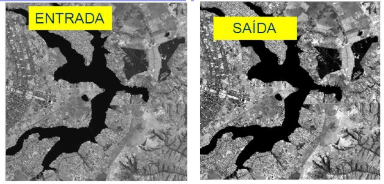
\includegraphics[width=.8\textwidth]{histograma}
	\caption{Exemplo de aplicação de equalização de  histograma.}
%	\fonte{\cite{lapix_escala}}
	\label{fig:histograma}
\end{figure}



\subsubsection{Segmentação}\label{subsubsec:segmentacao}

Em visão computacional, segmentação se refere ao processo recortar uma imagem digital, ou seja, recolher um conjunto de pixels, para simplificar, mudar a representação de uma imagem ou extrair áreas relevantes para facilitar a sua análise. 

Como resultado, cada um dos pixels em uma mesma região é similar com referência a alguma característica ou propriedade computacional, tais como cor, intensidade, textura ou continuidade. Este processo é pré requisito para que reconhecimentos de objetos tenham grandes chances de sucesso \cite{gonzalez_woods}.

\subsubsection{Classificação}\label{subsubsec:classificacao}

Segundo \cite{edinburgh_classifier}, classificação de imagem contextual é um tópico de reconhecimento de padrões em  Visão Computacional. Chama-se "contextual" pois significa que esta abordagem é focada na proximidade com os pixels e sua relação com o "classificador", (contemplado na seção \autoref{subsubsec:elem_haar}). É utilizado efetivamente na detecção de objetos e também pode ser aplicado para a detecção de faces em uma imagem.


%============================================================================================================


\section{Detecção de Faces com Classificadores Haar}\label{sec:deteccao}

Um classificador HAAR pode ser treinado para detectar vários tipos de objetos rígidos, definidos, como carros, motos ou partes do corpo humano como olhos ou boca, com altas taxas de sucesso. Não é muito eficiente em reconhecer objetos com ramos tipo arvores, mãos ou objetos camuflados ou contendo pouca textura, contorno e sub-regiões que variam em cor e iluminação \cite{drmathew_java_programming}.

Um classificador bem treinado pode envolver \textit{milhares} de fotos de alta qualidade com imagens positivas. Para a detecção de faces, isto significa imagens de reostos tiradas de perto que devem ter posições similares com muito pouca variação de fundo (\textit{background} \textit{variation}). Olhos bocas e narizes devem estar na mesma posição em todas as fotos, e estas devem ser do mesmo tamanho. Também é necessário treinar o classificador com um número similar de imagens negativas (isto é, sem rostos).

Existem diversas bibliotecas com classificadores pré-treinados para diferentes objetos, incluindo faces.


\subsection{As Características Haar (\textit{Haar Features}) }\label{subsubsec:elem_haar}

Os classificadores Haar (ou cacarcterísticas de haar, ou filtro haar) recebem esse nome pela sua similaridade com a \textit{Haar wavelet} (ou ondulação Haar), que consiste em uma sequência de funções quadradas redimensionadas que formam uma familia de ondulações das mais simples possíveis.

 \begin{figure}[h]
 	\centering
 	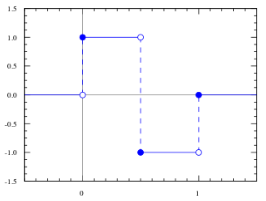
\includegraphics[width=.6\textwidth]{haarwavelet}
 	\caption{Um exemplo de \textit{Haar wavelet}}
 	%	\fonte{\cite{lapix_escala}}
 	\label{fig:haarwavelet}
 \end{figure}

Características Haar são basicamente imagens treinadas e usadas para achar objetos similares em outras imagens. Viola e Jones em seu algoritmo \textit{Haar Cascades} (contemplado na seção seguinte), por exemplo, utilizam classificadores retangulares. Cada classificador pode indicar a existência ou a ausência de uma característica em outra imagem. A maior motivação para o uso de características em um objeto ao invés do uso de pixel é que a velocidade da análise de uma imagem baseada no conjunto de sua principais características é muito maior do que a análise baseada sobre seus pixels, devido ao fato do numero de características ser substancialmente inferior em relação ao número de pixels \cite{gustavo_cascata}.

A \autoref{fig:haarfeatures} mostra um classificador Haar em ação.

 \begin{figure}[h]
	\centering
	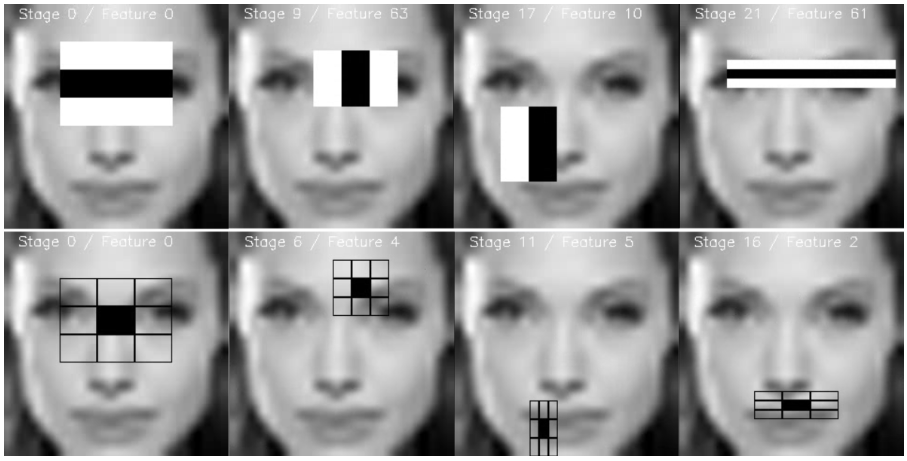
\includegraphics[width=.9\textwidth]{haarfeatures}
	\caption{Classificadores Haar representando características relevantes face}
	\fonte{Biblioteca OpenCV}
	\label{fig:haarfeatures}
\end{figure}

Estes padrões retangulares podem ser escalonados para que caracterísricas de diferentes tamanhos na imagem possam ser detectados usando a mesma abordagem.


\subsection{Algoritmo Viola-Jones (\textit{Haar Cascades Classifier}) }\label{subsubsec:violajones}

O \textit{framework} de detecção de objetos Viola-Jones, apelidado em inglês de \textit{Haar Cascades Classifier}, ou em português Cascata de Classificadores Haar \cite{gustavo_cascata}, foi o primeiro algoritmo de detecção a fornecer detecção de objetos com taxas de sucesso competitivas e em tempo real. Foi proposto em 2001 por Paul Viola e Michael Jones. Apesar de poder detectar uma variedade de classes de objetos, foi desenhada com o objetivo primordial de detectar faces.

Com a utilização das características Haar, o objetivo a ser alcançado é classificar corretamente um dado objeto a partir do conjunto de suas principais características. 

De acordo com \cite{drmathew_java_programming}, o algoritmo funciona com o uso de integrais que são rápidas e eficientes, possibilitando ainda reduzir drasticamente o número de atributos que precisam ser testados para decidir se a imagem contem um objeto (por exemplo uma face). O teste de atributos da imagem são organizados em "cascatas" (também pode ser representado por uma árvore binária), representando o uso das integrais iterativas.

O nó-raiz da árvore binária deve contér um valor representando o teste que se provou ser o melhor em encontrar um objeto durante o treino. Se uma imagem não é rejeitada por este valor teste entao a imagem segue para o nó com o segundo melhor valor de teste, e assim sucessivamente. Apenas se a imagem alcançar o fim de todos os nós (o fim da cascata ou da árvore) sem ser rejeitado, a imagem certamente deverá conter o objeto característico.

O grande ponto negativo é que este algoritmo também detecta os objetos que não são realmente os objetos que se tinha a intenção de detectar\cite{drmathew_java_programming}. Por exemplo, o desenho de um rosto certamente vai ser detectado com uma face original, e este desenho não precisa ser muito bem elaborado. As vezes uma disposição de sombras e regiões luminosas aleatórias podem er detectadas como objetos característicos .

Segundo \cite{gustavo_cascata}, os estágios dentro de uma cascata são criados através da combinação de funções de classificadores Haar previamente treinados. O principal objetivo do uso de cascatas é fazer com que seus estágios iniciais descartem um grande numero de regiões que contem o objetivo desejado, e estágios mais avançados sejam melhores em evitar um falso positivo na região analisada. 

A \autoref{fig:cascata} representa os $N$ estágios de uma cascata de classificadores. Cada um deles deve descartar ao máximo o número de regiões da imagem que não contém o objeto, a fim de diminuir a quantidade de processamento de outras sub-áreas da imagem original \cite{gustavo_cascata}.

 \begin{figure}[h]
	\centering
	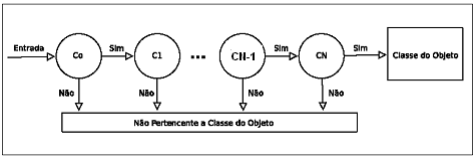
\includegraphics[width=.8\textwidth]{cascata}
	\caption{Cascata de classificadores com estágios (C0, C1, ..., Cn)}.
	\fonte{\cite{gustavo_cascata}}
	\label{fig:cascata}
\end{figure}

O processo para geração da cascata é guiado por um conjunto de metas de detecção e de desempenho. Na prática, uma arquitetura muito simples pode ser usada para produzir uma eficiente cascata de classificadores. O usuário pode informar as taxas mínimas aceitáveis e cada estágio da cascata é treinada junto ao conjunto de características Haar contando com cada vez mais elementos até que se atinjam as taxas de detecção de sucesso e falsos positivos. As taxas são encontradas testando o detector corrente sobre um conjunto de validação. Se a taxa de falsos positivos ainda não for atendida, então um novo estágio subsequente é ativado, coletando todas as falsas detecções encontradas \cite{gustavo_cascata}.

Para que o algoritmo possa detectar o objeto de interesse, é necessário que a imagem seja percorrida diversas vezes em várias direções, assim a cada iteração é analisado uma região de tamanho diferente, chamada \textbf{janela de busca} \cite{gustavo_cascata}. 

O usuário pode definir o tamanho desta janela que deve ser maior ou igual ao tamanho das imagens que foram treinadas na cascata, ou seja, se a cascata foi treinada com imagens positivas de 24x24 pixels, o tamanho mínimo da janela de busca deve seguir a mesma resolução \cite{gustavo_cascata}. As janelas devem funcionar em \textit{thread} (multiplas locações), sendo que \textit{n} janelas devem se deslocar no eixo X da imagem e \textit{m} janelas no eixo Y. A quantidade de janelas deve ser o suficiente para ocupar todo o espaço da imagem.

Outro valor que o usuário pode informar é número de detecções subsequentes necessários para que a região seja considerada a ter o objeto alvo. Reduzir este valor pode aumentar a velocidade de processamento, mas também aumenta as chances de taxas de falsos positivos \cite{drmathew_java_programming}.

O resultado do algoritmo são as posições dos objetos classificados com as características as quais se recebeu treinamento, podendo ser identificados na imagem.


%============================================================================================================


\section{\textit{EigenFaces} e Análise de Componentes Principais (ACP) }\label{sec:recog_faces}

O processo de reconhecimento de faces depende de uma fase de treinamento precedente envolvendo imagens faciais com suas identidades associadas. Imagens típicas de treinamento são mostradas na \autoref{fig:trein_img}.
\begin{figure}[h]
	\centering
	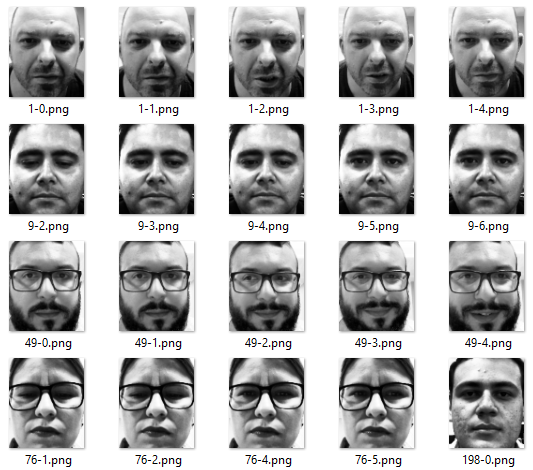
\includegraphics[width=.7\textwidth]{trein_img}
	\caption{Exemplo de imagens típicas de treinamento.}
	%	\fonte{\cite{img-digital-willians}}
	\label{fig:trein_img}
\end{figure}

É importante que as imagens sejam todas colhidas e orientadas de maneira similar, para que as variações entre as imagens sejam causadas por diferenças entre as faces e não por diferenças  em plano de fundo ou posição facial. Também deve haver uniformidade na posição, clareamento, tamanho e resolução da imagem. É recomendado incluir várias imagens da mesma face mostrando diferentes expressões, como sorrindo ou abrindo a boca. A relação da imagem com o indivíduo pode ser feita de diversas maneiras, uma delas é codificar alguma chave único para o indivíduo junto ao nome da imagem \cite{drmathew_java_programming}. 



O processo de treinamento cria as \textit{EigenFaces}, como mostra a \autoref{someeigen} explicada na  \autoref{subsec:treinrecface}, que são composições das imagens de treinamento que tem a propriedade de acentuar elementos que podem ser distinguidos mais facilmente pelo algoritmo. Uma imagem de face pode gerar várias \textit{Eigenfaces}. As imagens de treino da face podem ser representadas por uma sequência de "pesos" (p1, p2, p3, p4, p5, p6), como ilustra a figura \autoref{fig:eigenpeso}.

\begin{figure}[h]
	\centering
	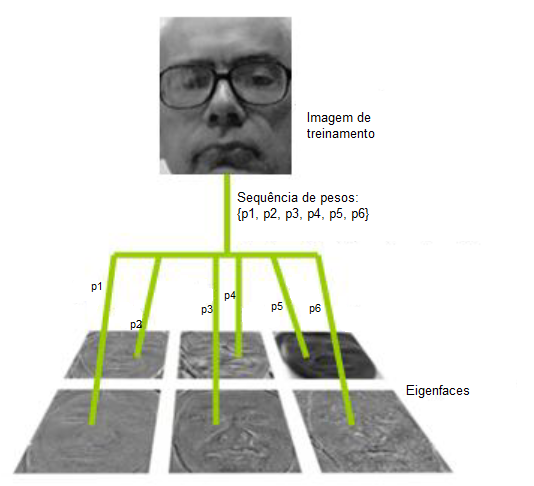
\includegraphics[width=.7\textwidth]{eigenpeso}
	\caption{Exemplo de uma imagem de treinamento representada em uma sequência de pesos de engenfaces.}
	\fonte{Adapdato de \cite{drmathew_java_programming}}
	\label{fig:eigenpeso}
\end{figure}

O objetivo é que a imagem de treinamento pode ser decomposta por uma soma dos pesos das multiplas \textit{engeifaces}, sendo todos estes pesos salvos como uma sequência.

Nem todas as eigenfaces são igualmente importantes - algumas pode contar elementos faciais mais importantes para distinguir faces. Isto quer dizer que não é necessário utilizar todas as eigenfaces para reconhecer uma face, o que permite que uma imagem seja representada por uma pequena quantidade de eigenfaces, o que ocupa menos espaço e torna a execução do algoritmo mais rápida. O ponto negativo é que com menos pesos, a probabilidade de se perder importantes elementos faciais também aumenta\cite{drmathew_java_programming}.

Outra maneira de se entender a relação entre eigenfaces e as imagens é representa-las em um plano cartesiado multidimensional (ou um \textit{eigenspace}), como mostra a \autoref{fig:eigenpeso_axis}.

\begin{figure}[h]
	\centering
	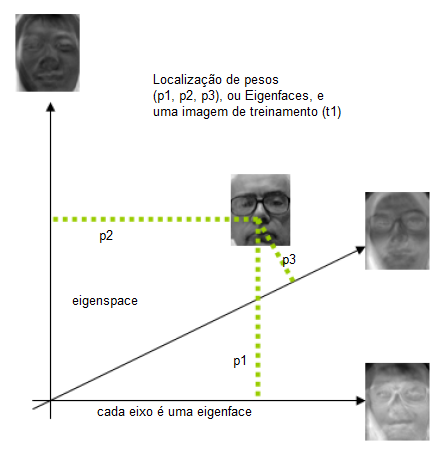
\includegraphics[width=.7\textwidth]{eigenpeso_axis}
	\caption{Exemplo de eigenfaces representadas em um plano cartesiano (\textit{eigenspace})de 3 dimensões. }
	\fonte{Adapdato de \cite{drmathew_java_programming}}
	\label{fig:eigenpeso_axis}
\end{figure}

Os pesos agora podem ser observados como as coordenadas da imagem de treinamento em um plano cartesiano multidimensional (\textit{eigenspace}). Na \autoref{fig:eigenpeso_axis}, existem apenas 3 eixos representando as eigenfaces p1, p2 e p3, porém se houvessem 10 eigenfaces, haveria 10 eixos neste plano cartesiano.

Após o processo de treinamento das faces vem o processo de reconhecimento. Neste novo processo, uma nova imagem para reconhecimento deve ser decomposta em eigenfaces (na mesma maneira da \autoref{fig:eigenpeso}). A sequência de pesos resultante é comparada com cada sequência de pesos que foram treinadas previamente, e o nome associado com o as características mais próximas dos eigenfaces treinados é associado \cite{drmathew_java_programming}.

Em outras palavras, em termos de \textit{engenspaces}, a nova imagem é posicionada no plano cartesiano com suas próprias coordenadas (pesos). Então uma técnica de medida de distância (usualmente a distância Euclidiana, que será abordada na \autoref{subsec:eigenacp}) é utilizada para encontrar e figura de treinamento correspondente mais próxima. Sendo assim, uma distância Zero seria uma correspondência (reconhecimento) perfeita \cite{drmathew_java_programming}. A \autoref{eigencartesiano} na \autoref{subsec:treinrecface} ilustra este processo.

As Eigenfaces são geradas utilizando um procedimento matemático chamado Análise de Componentes Principais - ACP (em inglês Principal Components Analysis - PCA). Esta técnica acentua as similaridades e as diferenças nos dados. 


%=======================================================================================================================

\subsection{Análise de Componentes Principais (ACP)}\label{subsec:acp}

Para que esta técnica seja explicada, será utilizado vetores de valores numéricos: o vetor \textit{x} e \textit{y}, como mostra a \autoref{tabelaxy}.

\begin{table}[h]
	\centering
	\caption{Dados dos vetores \textit{x} e \textit{y}.}
	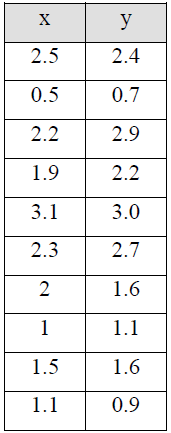
\includegraphics[width=.15\textwidth]{tabelaxy}
	\fonte{\cite{drmathew_java_programming}}
	\label{tabelaxy}
\end{table}

Os dados de \textit{x} e \textit{y} poderiam representar a altura de estudantes, preços de frutas, ou valores numéricos extraídos de uma imagem, por exemplo. O objetivo da demonstração é acentuar as diferenças e similaridades entre os dois vetores de dados em uma abordagem numérica \cite{drmathew_java_programming}. 

Para tal, medidas estatísticas como média e desvio padrão (uma medida que tem o objetivo de espalhar valores acerca da média). Variância é outra medida de espalhamento, que é igual ao desvio padrão ao quadrado:

\begin{figure}[h]
	\centering
	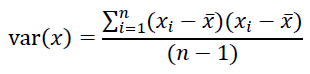
\includegraphics[width=.3\textwidth]{variancia}
%	\caption{Exemplo de eigenfaces representadas em um plano cartesiano (\textit{eigenspace})de 3 dimensões. }
%	\fonte{Adapdato de \cite{drmathew_java_programming}}
	\label{fig:variancia}
\end{figure}

A variável \textit{n} é o número de itens dos vetores (10 de acordo com a \autoref{tabelaxy}), e $\bar{x}$  é a média dos valores d conjunto de dados.

Contudo, a média e a variância fornecem informação apenas sobre a forma dos dados em um único vetor (por exemplo, e média e a variância do vetor \textit{x}), sendo que o objetivo é quantificar as diferenças \textbf{entre} os dois vetores \cite{drmathew_java_programming}.  Justamente a covariância é uma medida estatística, generalizada da variância, que compara dois conjuntos de dados \cite{drmathew_java_programming}:

\begin{figure}[h]
	\centering
	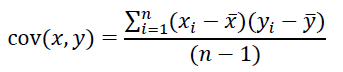
\includegraphics[width=.3\textwidth]{covariancia}
	%	\caption{Exemplo de eigenfaces representadas em um plano cartesiano (\textit{eigenspace})de 3 dimensões. }
	%	\fonte{Adapdato de \cite{drmathew_java_programming}}
	\label{fig:variancia}
\end{figure}

Se a fórmula da covariância for aplicada nos dados dos vetores \textit{x} e \textit{y} dados na \autoref{tabelaxy}, o resultado será 0.6154. A parte em que se deve estar atendo é o sinal: se for negativo significa que quando um vetor aumenta em dados, o outro diminui. Quando o valor é positivo, que é o caso, então os dois conjuntos de dados aumentam juntas. Para ilustrar este conceito, na \autoref{fig:graphxy} plota-se os valores correspondentes dos vetores \textit{x} e \textit{y} como pontos em um gráfico \cite{drmathew_java_programming}.


\begin{figure}[h]
	\centering
	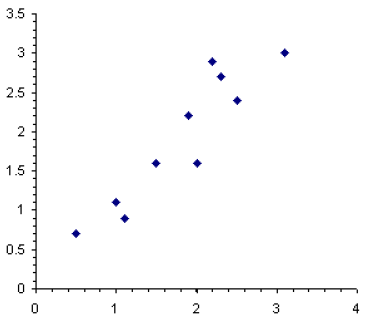
\includegraphics[width=.4\textwidth]{graphxy}
	\caption{Plotagem dos valores de \textit{x} e \textit{y}.}
	\fonte{Adapdato de \cite{drmathew_java_programming}}
	\label{fig:graphxy}
\end{figure}

Se houverem mais de dois vetores (por exemplo o vetor \textit{x}, \textit{y} e \textit{z}) então a covariância deve ser calculada entra todas os conjuntos de dados, ou seja, calculando cov(x, y), cov(x, z) e cov(y, z). 

Não há necessidade de calcular cov(y, x), cov(z, x) e cov(z, y) sendo que a definição da equação garante que cov(A, B) é igual a cov(B, A) .

A maneira padrão de armazenar a covariância entre múltiplos vetores de dados é por uma matriz onde os conjuntos de dados tornam-se os índices das colunas e linhas. Por exemplo, a covariância para os conjuntos de dados x,y e z se tornariam uma matriz de dimensões 3x3 \cite{drmathew_java_programming}:

\begin{figure}[h]
	\centering
	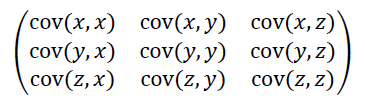
\includegraphics[width=.3\textwidth]{covmatrix}
	%	\caption{Exemplo de eigenfaces representadas em um plano cartesiano (\textit{eigenspace})de 3 dimensões. }
	%	\fonte{Adapdato de \cite{drmathew_java_programming}}
	\label{fig:covmatrix}
\end{figure}

Na diagonal principal, pode-se observar que a covariância é entre o conjunto de dados a própria covariância, que é equivalente à variância nestes dados. Podemos provar isto comparando a variância de x ( var(x) ) e a covariância de x com x ( cov(x) ). A matriz também apresenta simetria em volta da diagonal principal. 

Os conjuntos de dados \textit{x} e \textit{y} da \autoref{tabelaxy} seriam representados em uma matriz de dimensões 2x2:

\begin{center}
	$\begin{pmatrix} 0.6166 & 0.6154 \\ 0.6154 & 0.7166 \end{pmatrix}$
\end{center}


A matriz de covariância é um meio útil de demonstrar a relação entre os conjuntos de dados, mas deve-se obter ainda mais informações para que sejam geradas as \textit{eigenfaces} calculando dois vetores que serão contemplados na seção seguinte: \textit{eigenvectors} e \textit{eigenvalues}.

\subsection{ACP E \textit{Eigenfaces}}\label{subsec:acp-eigen}

Para que as eigenfaces sejam geradas, deve-se transformar a covariância ou outros conjuntos de dados chamados de \textit{eigenvectors} e \textit{eigenvalues}.

Segundo \cite{drmathew_java_programming}, o \textit{eigenvector} é um vetor de valores ordinário que quando multiplicado por uma dada matriz, muda de magnitude, enquanto que \textit{eigenvalue} é apenas um termo para esta magnitude. 

Por exemplo, dada a matriz:

\begin{center}
	$\begin{pmatrix} 2 & 3 \\ 2 & 1 \end{pmatrix}$
\end{center}

O eigenvector para esta matriz é $\begin{pmatrix} 3 \\ 2\end{pmatrix}$, pois quando multiplicado pela matriz acima, o mesmo vetor é retornado o mesmo vetor é retornado se multiplicado por 4:

\begin{center}
	$\begin{pmatrix} 2 & 3 \\ 2 & 1 \end{pmatrix}$ $\times$ $\begin{pmatrix} 3 \\ 2 \end{pmatrix}$ $=$ $4$ $\times$ $\begin{pmatrix} 2 \\ 3\end{pmatrix}$
\end{center}

Sendo assim, 4 é o \textit{eigenvalue} para o \textit{eigenvector}  $\begin{pmatrix} 3 \\ 2\end{pmatrix}$.

Os eigenvectores podem ser encontradas apenas para matrizes quadradas, porém nem todas. Para uma dada matriz n x n, se realmente houver eigenvectores, haverá n. A matriz 2x2 usada de exemplo acima tem dois eigenvetores (e seus valores eigenvalues correspondentes).

A relação eigenvalue pode ser escrita matematicamente como: 

 $\Lambda$ $\nu$  $=$  $\lambda$ $\nu$  

onde $\Lambda$ é a matriz quadrada, $\nu$ é um eigenvetor para A e o valor $\lambda$ é um eigenvalue.

Para usa-los no algoritmo PCA, os eigenvetores devem ser normalizados para que todos eles tenham a mesma unidade de tamanho. Isto é, o eigenvetor acima, $\begin{pmatrix} 3 \\ 2\end{pmatrix}$, tem a unidade de tamanho "falso" de  $\sqrt[]{(3^2 + 2^2)}$ $=$ $\sqrt[]{13}$. Se o vetor for dividido por este valor resultara em um tamanho de unidade \cite{drmathew_java_programming}:

\begin{center}
	$\begin{pmatrix} 3 \\ 2 \end{pmatrix}$ 
	$\div$  
	$\sqrt[]{13}$ $=$ 
	$\begin{pmatrix} 3 / \sqrt[]{13} \\ 2/\sqrt[]{13} \end{pmatrix}$
\end{center}

Se recuperarmos a matriz de covariância que geramos acima:

\begin{center}
	$\begin{pmatrix} 0.6166 & 0.6154 \\ 0.6154 & 0.7166 \end{pmatrix}$
\end{center}

pode-se observar que, com é uma matriz 2x2, possui dois eigenvetores e eigenvalues:

\begin{center}
$\begin{pmatrix} -0.7352 \\ 0.6779 \end{pmatrix}$  e 0.049

$\begin{pmatrix} 0.6779 \\ 0.7352 \end{pmatrix}$  e 1.284
\end{center}

Ambos os eigenvetores possuem unidade de tamanho.

\subsubsection{Utilizando Eigenfaces como Componente Principal}\label{subsec:eigenacp}

Observando novamente a plotagem dos vetores x e y contemplados na \autoref{fig:graphxy}, se a média destes conjuntos de dados ($\bar{x}$ e $\bar{y}$) for subtraído de seus valores, estes dados então seriam \textbf{normalizados}. Isto também quer dizer que as linhas que representam os vetores \textit{x} e \textit{y} são transladados para o centro como mostra a \autoref{fig:graphxy2}. 

\begin{figure}[h]
	\centering
	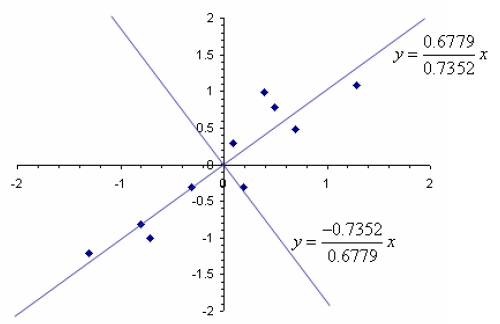
\includegraphics[width=.5\textwidth]{graphxy2}
	\caption{Plotagem normalizada dos dados de \textit{x} e \textit{y} com eigenvetores.}
	\fonte{\cite{drmathew_java_programming}}
	\label{fig:graphxy2}
\end{figure}

Os dois engenvetores pode ser adicionados ao gráfico como linhas convertendo os vetores em equações. 
$\begin{pmatrix} -0.7352 \\ 0.6779 \end{pmatrix}$ torna-se $y$ $=$ $\frac{-0.7352}{0.6779}$$x$  e $\begin{pmatrix} 0.6779 \\ 0.7352 \end{pmatrix}$ torna-se $y$ $=$ $\frac{0.6779}{0.7352}$$x$.

Os dados normalizados e as duas equações são ilustradas na \autoref{fig:graphxy2} como linhas azuis. 

Observa-se que na \autoref{fig:graphxy2} demonstra como os eigenvectores acentuam as relações entre os conjuntos de dados- os vetores indicam como os conjuntos de dados se espalham nas coordenadas do espaço cartesiano. Este espalhamento facilita a distinção dos dados \cite{drmathew_java_programming}.

Dos dois eigenvetores marcados em azul, a linha $\frac{0.6779}{0.7352}$$x$ é a mais útil, pois os dados estão mais espalhados acerca do trajeto desta linha. Isto pode ser confirmado numericamente observando o eigenvalue associado com seu eigenvetor: o eigenvalue (1.284) é um melhor indicador de espalhamento pois é o maior dentre os dois eigenvalues.

A outra linha, $\frac{-0.7352}{0.6779}$$x$, contribui com a informação demonstrando como os dados são espaçados para direita ou esquerda do eigenvetor principal (a linha $\frac{0.6779}{0.7352}$$x$). Entretanto, trata-se de um componente menos importante no espalhamento de dados, assim como indica seu eigenvalue (0.049) \cite{drmathew_java_programming}.

O eigenvetor com o maior eigenvalue (no caso a linha $\frac{0.6779}{0.7352}$$x$, ou o vetor $\begin{pmatrix} 0.6779 \\ 0.7352 \end{pmatrix}$) é chamado de \textbf{componente principal} do conjunto de dados. Isto é, os eigenvetores e eigenvalues são efetivamente utilizados para performar uma análise de componente principal nos conjuntos de dados \cite{drmathew_java_programming}.

Todos os eigenvetores extraídos da matriz são perpendiculares. Isto significa que é possível rotacionar (talvez refletir) os dados para que os eigenvetores tornem-se alinhados com os eixos. Se este componente principal $\begin{pmatrix} 0.6779 \\ 0.7352 \end{pmatrix}$ for rotacionado e refletido para que seja alinhado com o eixo y, resulta-se em uma plotagem mostrada na \autoref{fig:graphxy3}:

\begin{figure}[h]
	\centering
	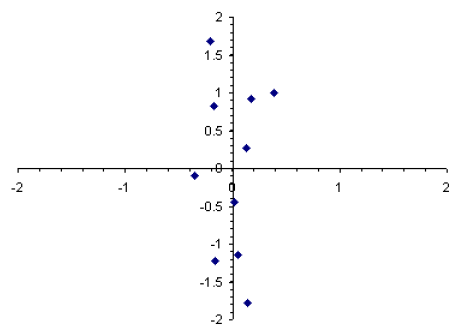
\includegraphics[width=.5\textwidth]{graphxy3}
	\caption{Versão rotacionada e refletida da \autoref{fig:graphxy2}}
	\fonte{\cite{drmathew_java_programming}}
	\label{fig:graphxy3}
\end{figure}

Observando a \autoref{fig:graphxy3}, o ponto mais próximo da origem se situa na coordenada (0.13, 0.27). Pode-se afirmar que também que este ponto tem uma sequência de pesos relativos a cada eigenvetor, no caso, a sequência {0.13, 0.27}.

Tanto a denotação de coordenadas quanto a de pesos pode ser usada para representar as eigenfaces - como contemplado anteriormente, na \autoref{fig:eigenpeso} foi dado o exemplo em que uma imagem é uma sequência de pesos de seis eigenfaces, enquanto que, alternativamente, na  \autoref{fig:eigenpeso_axis} é representada em coordenadas de um plano cartesiado de 3 dimensões, sendo que cada eixo é definido por uma \textit{eigenface} (ou \textit{eigenvector}).

\subsubsection{O Reconhecimento}\label{subsec:reconhecimento}

O processo de reconhecimento consiste em recolher novos conjutos de dados (no caso, uma nova face), e utilizando os dados processados até agora e representados na \autoref{fig:graphxy3}, deve-se comparar os dois novos conjuntos de dados (a nova face e os eigenfaces ou eigenvetores) fazendo uso de medidas de distância. 

Existem algumas técnicas de medidas de distância, dentre elas, há uma simples chamada \textbf{Distância Euclidiana}. Esta medida nada mais é do que a distância mínima entre dois pontos no espaço (uma linha reta). A distância euclidiana entre os pontos $P = (p_1, p_2, ..., p_n)$ $Q = (q_1, q_2, ..., q_n)$ é definida como:

\begin{center}
	$\sqrt[]{(p_1 - q_1)^2 + (p_1 - q_1)^2 + ... + (p_n - q_n)^2}$ $=$ $\sqrt[]{ \sum_{i=1}^{n} (p_i - q_i)^2 }$ 
\end{center}

O resultado desta medida é utilizada para calcular a taxa de sucesso de uma comparação, sendo assim uma distância nula representaria uma equivalência perfeita.

Contudo, em aplicações na vida real, deve-se reduzir o tamanho dos dados, pois existem informações irrelevantes e a tarefa de reconhecimento pode ser executada mais rapidamente enquanto retém informações suficientes para distinguir entre os pontos quando comparados com os novos conjuntos de dados.

A técnica consiste em reter todas as coordenadas dos dados, mas reduzir a dimensionalidade do eigenspace, isto é, subtrair o número de eixos do plano cartesiano. Este processo é equivalente a subtrair algumas eingenfaces, mas como citado anteriormente, os enigenvalues de menor intensidade não tem influência no espalhamentos dos dados no plano, sendo pouco significativos para o reconhecimento, e portanto podem ser removidos.

Portanto, os dados mostrados na  \autoref{fig:graphxy3} possuem os seguintes eigenvetores e eigenvalores:

\begin{center}
	$\begin{pmatrix} -0.7352 \\ 0.6779 \end{pmatrix}$  e 0.049
	
	$\begin{pmatrix} 0.6779 \\ 0.7352 \end{pmatrix}$  e 1.284
\end{center}

Observando que o primeiro \textit{eigenvector} foi rotacionado em direção ao eixo $x$, e o segundo \textit{eigenvector} em direção ao eixo $y$, se o primeiro \textit{eigenvector} que contribui muito pouco para a informação de espalhamento (devido ao seu pequeno \textit{eigenvalue}) for descartado junto ao seu eixo, os dados deste \textit{eigenvcetors} são projetados para o eixo $y$, resultando na plotagem da \autoref{fig:graphxy4}

\begin{figure}[h]
	\centering
	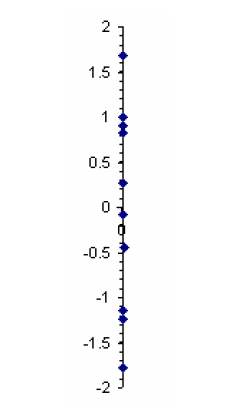
\includegraphics[width=.2\textwidth]{graphxy4}
	\caption{Dados da \autoref{fig:graphxy3} projetados em direção ao eixo y.}
	\fonte{\cite{drmathew_java_programming}}
	\label{fig:graphxy4}
\end{figure}


Apesar dos eixos serem eliminados, seus dados ainda estão presentes e espalhados o suficiente para que o novo conjunto de dados seja comparado com o uso da distância euclidiana.

Considerando que um novo conjunto de dados adicionado com os valores do vetor \textit{z} = (2.511, 2.411), e estes conjuntos passarem pelos mesmos processos que os vetores \textit{x} e \textit{y}, e por fim normalizado e projetado assim como mostra a \autoref{fig:graphxy2} e \autoref{fig:graphxy3}, plotando-o no mesmo espaço resulta na \autoref{fig:graphxy5}.

\begin{figure}[h]
	\centering
	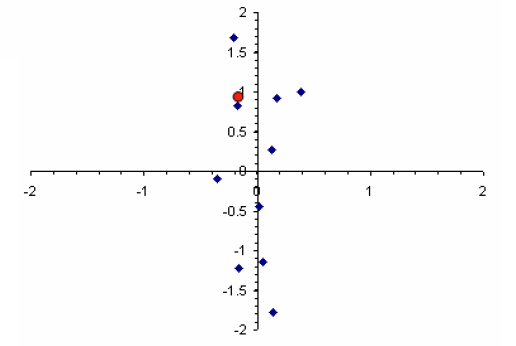
\includegraphics[width=.5\textwidth]{graphxy5}
	\caption{Plotagem dos novos dados com os dados de treino transformados.}
	\fonte{\cite{drmathew_java_programming}}
	\label{fig:graphxy5}
\end{figure}

A \autoref{fig:graphxy5} é a mesma que a \autoref{fig:graphxy3} com a adição de um novo ponto vermelho que indica a ccoordenada do novo conjunto de dados do vetor \textit{z}, posicionada logo acima do ponto (-0.1751, 0.8280), que por sua vez começou como um ponto de treinamento de pesos (2.5, 2.4), informada nos conjuntos de dados \textit{x} e \textit{y}. Isto quer dizer que o novo conjunto de dados \textit{z} (2.511, 2.411) possui a menor distância euclidiana com o conjunto de treinamento (2.5, 2.4). 

A real vantagem dos eigenvetores é quando a dimensionalidade do espaço (eigenspace) torna-se extremamente grande. No presente exemplo foi utilizado uma dimensionalidade dois, enquanto que em aplicações reais com imagem os eixos podem aumentar para valores como 40 mil \cite{drmathew_java_programming}.

Com tamanha dimensão e portanto, quantidade de eixos, como citado anteriormente, pode-se eliminar alguns eixos dependendo de seus valores eingenvalues (se forem pequenos, podem ser considerados dispensáveis). Se por uma hipótese isto for feito neste exemplo incluindo o novo conjunto dados \textit{z}, a plotagem do resultado seria como na \autoref{fig:graphxy6} abaixo:

\begin{figure}[h]
	\centering
	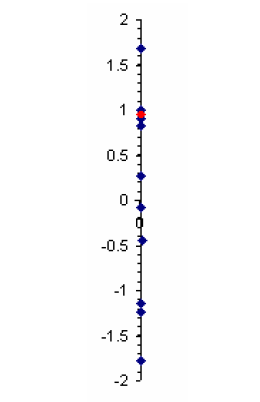
\includegraphics[width=.2\textwidth]{graphxy6}
	\caption{Plotagem dos conjuntos de dados \textit{x}, \textit{y} e \textit{z}, trasnformados e projetados no eixo do Componente Principal}
	\fonte{\cite{drmathew_java_programming}}
	\label{fig:graphxy6}
\end{figure}

A \autoref{fig:graphxy6} é similar à \autoref{fig:graphxy4} com exceção do ponto vermelho (novo dado). Pode-se observar nesta figura o problema potencial em se reduzir a dimensionalidade: a probabilidade de erros aumenta tornando difícil de decidir qual ponto de treinamento é que possui a menor distância euclidiana. Outro fator da equação da distância euclidiana é que se utiliza de um parâmetro para definir quando dois pontos estão perto. Se um valor alto é definido então diversos pontos podem estar dentro do alcance aceitável do novo dado \cite{drmathew_java_programming}.


\subsection{EigenVectors para EigenFaces}\label{subsec:vectoface}

O transformação dos valores numéricos gerados na ACP para imagens EigenFaces nao são necessário para os algoritmos apresentados. Essa transformação serve apenas para satisfazer olhos humanos, ou seja, uma tentativa de observar em imagens os valores gerados pela teoria.


Essencialmente, deve-se converter a imagem para um conjunto de dados, como os vetores $ x $ e $ y $ apresentados na \autoref{tabelaxy}, e performar o algoritmo ACP como descrito anteriormente. A translação de uma imagem para um conjunto de dados é feita tratando esta como um vetor de duas dimensões, e em seguida mapear para um vetor unidimensional como sugere a \autoref{fig:2dto1d}:

\begin{figure}[h]
	\centering
	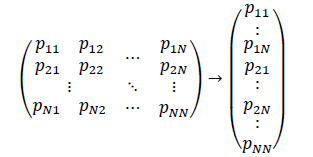
\includegraphics[width=.38\textwidth]{2dto1d}
	\caption{Conversão de imagem para conjunto de dados. A variável $P$ seria a representação de um pixel.}
	\fonte{\cite{drmathew_java_programming}}
	\label{fig:2dto1d}
\end{figure}

Supondo que a imagem tem o tamanho de 200x200 pixels em escala de cinza, o conjunto de dados resultante residirá em um \textit{eigenspace} de 40 mil dimensões, o que acarretará na geração de 40 mil \textit{eigenvectors}, cuja a maioria possui um \textit{eigenvalue} desconsiderável ou insignificante, podendo assim ser descartados. Isto facilitará o processamento da imagem e a utilização da técnica. 

Em geral, supondo que uma imagem quadrada em escala de cinza tem o tamanho de  $ N $ pixels, então $N^2$ eigenvetors serão criados. No seguinte exemplo, será assumido que existem $ M $ imagens:

A técnica consiste em "dividir" a matriz de covariância que é ($ N^2 x N^2 $) em duas matrizes de ($ N^2 x M $) e ($ M x N^2 $). 



%============================================================================================================

\section{Considerações Finais}\label{sec:revbib_consid_finais}

Neste capítulo foram apresentados os conceitos necessários para o entendimento de todo o processo de Reconhecimento de Faces, constituído de outros sub processos como aquisição de imagem e vídeo, processamento e  classificação de imagens, detecção da face, treinamento e por fim o reconhecimento efetivo da face.

Os algoritmos de detecção de face Viola-Jones, e o de reconhecimento de faces EigenFaces que utiliza o método matemático ACP (Análise de Componentes Principais), foram detalhados na ordem sequêncial de seus processos utilizando exemplos.

No próximo capítulo abordará o plano de materiais e métodos elaborado a partir do conhecimento adquirido no \autoref{ch:rev-bibs}.
























% !TeX encoding = UTF-8

\chapter{MATERIAIS E MÉTODOS}\label{ch:materiais-metodos}
Após os estudos realizados sobre processamento e classificação de imagens, sobre o algoritmo de detecção \textit{Haar-cascades} e o de reconhecimanto \textit{EigenFaces} contemplado no capítulo passado, é necessário definir o material e meio para desenvolver o sistema aqui proposto.

Este capítulo apresentará os materiais e metodos que serão utilizados para o desenvolvimento do sistema proposto neste trabalho.


\section{MATERIAIS}\label{sec: tec-ferramenta}
As seguintes seções irão detalhar os equipamentos que serão usados para o desenvolvimento do sistema e as tecnologias de software escolhidas baseado na revisão bibliográfica realizada e na experiência do autor.

\subsection{Hardwares}\label{sub-hardw}
Lista-se a seguir, os equipamentos necessários para a realização deste trabalho:

\begin{itemize}
	
	\item Câmera digital do tipo \textit{Web} (\textit{Webcam}) de 720p de resolução (ou 1280x720 \textit{pixels});
	\begin{itemize}
		\item será utilizada para captar o vídeo analógico e disponibilizá-lo no formato digital
	\end{itemize}

	\item Microcomputador pessoal com processador Intel i7, 32 gigabytes de memória, e placa de vídeo externa de 16 megabytes (alto rendimento);
	\begin{itemize}
		\item será utilizado como principal instrumento de desenvolvimento
	\end{itemize}
	
	\item Microcomputador pessoal do tipo notebook com processador Intel i3 de versão antiga, 2 gigabytes de memória, sem placa de vídeo externa, utilizando a própria memória RAM para renderização (baixo à médio rendimento);
	\begin{itemize}
		\item será utilizado como instrumento de desenvolvimento secundário, para testar questões de consumo de memória e processamento (desempenho)	
	\end{itemize}
	
\end{itemize}

Estes \textit{hadwares} são considerados suficientes para a realização deste trabalho.

\subsection{Softwares}\label{sub-softw}
As subseções seguintes irão citar e detalhar as tecnologias que serão utilizadas para a implementação do trabalho aqui proposto,  descrevendo a maneira que serão utilizados.

\subsubsection{Linguagem Java}\label{subsec:java}
A tecnologia Java é usada para desenvolver aplicativos para uma ampla variedade de ambientes, de dispositivos consumidores a sistemas corporativos heterogêneos \cite{ibm_java}. 

A linguagem Java deriva da linguagem C, portanto suas regras de sintaxe assemelham-se às regras de C. Por exemplo, os blocos de códigos são modularizados em métodos e delimitados por chaves ({ e }) e variáveis são declaradas antes que sejam usadas \cite{ibm_java}. 

Estruturalmente, a linguagem Java começa com pacotes. Um pacote é o mecanismo de \textit{namespace} da linguagem Java. Dentro dos pacotes estão as classes e dentro das classes estão métodos, variáveis, constantes e mais \cite{ibm_java}.

Java é uma linguagem Orientada a Objetos. A Programação Orientada a Objetos (POO) diz respeito a um padrão de desenvolvimento que consiste na representação de cada elemento em termos de um objeto, ou classe. Esse tipo de representação procura aproximar o sistema que está sendo criado ao que é observado no mundo real, e um objeto contém características e ações, assim como vemos na realidade \cite{dev_poo}. 

O Java possui classes prontas para a solução dos mais diversos problemas. A seguinte lista descreve as classes ou pacotes que este trabalho fará uso, dentre outras:

\begin{itemize}
	
	\item Pacote \textbf{\textit{java.swing}} e \textbf{\textit{java.awt}}: possui classes para a construção da interface (ou \textit{front-end}) do sistema. Botões, janelas, manipulação de eventos e outros componentes visuais;
	
	\item Pacote \textbf{\textit{java.io}}: utilizado para manipular entrada e saida de informações, manipulação de arquivos e pastas, etc;
	
	\item Pacote \textbf{\textit{java.util}}: possui classes de estrutura e manipulação de listas e filas, além uma variedade de classes úteis para problemas esporádicos;
	
	\item outros pacotes utilizados casualmente de acordo com a necessidade como o \textbf{\textit{java.lang}} provê classes que são fundamentais para a programação Java, por exemplo as classes de criação e execução de \textit{threads};	
	
\end{itemize}

\subsubsection{Biblioteca OpenCV, JavaCV e JavaCPP}\label{subsec:bib_opencv}

A biblioteca \textbf{OpenCV} (Open Source Computer Vision Library) foi originalmente desenvolvida pela Intel em 2000 e hoje é uma biblioteca multiplataforma, totalmente livre ao uso acadêmico e comercial, para o desenvolvimento de aplicativos na área de Visão computacional \cite{opencv}.

Seu código foi escrito em nas linguagens C e C++, porém possui interface para várias outras linguagens como Python, Visual Basic, Java, dentre outras. Incorpora algoritmos para a resolução de vários problemas na área de visão computacional, inclusive o algoritmo Haar-Cascades contemplados na \autoref{subsubsec:violajones}, o qual será utilizado.

A biblioteca \textbf{JavaCPP}, atualmente mantida pelo grupo ByteDeco, é considerada uma \textit{bridge} ("ponte") entre a linguagem C++ e Java, disponibilizando classes de configurações e interfaces para várias bibliotecas escritas em C++, inclusive a OpenCV \cite{javacpp}.

Por sua vez, a biblioteca \textbf{JavaCV},inicialmente desenvolvida pela Google e agora mantida pelo grupo 1ByteDeco, utiliza as interfaces e \textit{wrapers} da biblioteca JavaCPP e provê classes úteis que podem ser usadas para manipular a  OpenCV de maneira mais fácil para plataforma Java \cite{javacv}. Também oferece drivers de aceleração gráfica que otimizam o funcionamento da OpenCV na plataforma Java, dentre outras utilizades.

Estas três bibliotecas funcionam de maneira conjunta para resolver a problemática de aquisição, processamento de imagens, e classificação de objetos, e será utilizada neste trabalho.

A lista a seguir disponibiliza e detalha os principais pacotes, classes e métodos ou funções que se fará uso destas bibliotecas de desenvolvimento. As definições de suas funções foram retiradas das documentações dispostas nos \textit{links} de \cite{opencv}, \cite{javacv} e \cite{javacpp}: 

\begin{itemize}
	\item Pacotes/classes:
	\begin{itemize}
		\item \textit{\textbf{javacpp.opencv\_core.CvMemStorage}}: classe que representa um bloco de memória para armazenamento de vários componentes da OpenCV. Trata problemas alocação e desalocação de memória;
		
		\item \textbf{\textit{javacpp.opencv\_core.CvRect}}: classe utilizada para representar um segmento de uma imagem com pontos x e y, altura e largura do segmento;
		
		\item \textbf{\textit{javacpp.opencv\_core.CvSeq}}: classe que representa uma lista (ou sequência) de classes do tipo \textit{CvRect};
		
		\item \textbf{\textit{javacpp.opencv\_core.IplImage}}: utilizada para representar uma imagem no fomrato \textit{raster};
		
		\item \textbf{\textit{javacv.VideoInputFrameGrabber}}:	classe responsável por estabelecer conexão com câmeras conectadas a um dispositivo (microcomputador, por exemplo);

		\item \textbf{\textit{javacv.FrameGrabber}}: esta classe tem a função de monitorar o fluxo de \textit{frames} de uma \textit{webcam} conectada a partir da classe \textit{VideoInputFrameGrabber} e disponibilizar uma imagem advinda deste fluxo quando requisitado;		
			
		\item \textbf{\textit{javacv.Java2DFrameConverter}}: tem a função de converter as classes de representações de imagens \textit{javacpp.opencv\_core.IplImage} e \textit{java.awt.image};
		
		\item \textbf{\textit{javacv.OpenCVFrameConverter}}: tem a função de converter as classes de representações de imagens \textit{javacpp.opencv\_core.IplImage} e \textit{javacv.Frame}, disponibilizada pela classe \textit{FrameGrabber} acima listada;
		
		\item \textbf{\textit{javacpp.opencv\_objdetect.CvHaarClassifierCascade}}: classe que contém as configurações e o algoritmo de classificação Haar-Cascades, utilizado para a detecção de objetos (ou faces);
	\end{itemize}

	\item Métodos ou funções:
	\begin{itemize}		
		\item \textbf{\textit{javacpp.opencv\_core.cvClearMemStorage}}: esta função desaloca o espaço de memória utilizada pela classe \textit{CvMemStorage} listada acima;
		
		\item \textbf{\textit{javacpp.opencv\_core.cvCreateImage}}: responsável por criar objetos da classe \textit{IplImage}, aceitando parâmetros como produndidade de cores, tamanho da imagem, dentro outros;
		
		\item \textbf{\textit{javacpp.opencv\_core.cvReleaseImage}}: este método libera o espaço de memória ocupado pelos objeto das classe \textit{IplImage};

		\item \textbf{\textit{javacpp.opencv\_core.cvGetSeqElem}}: manipula objetos da classe \textit{CvSeq} listada acima;
		
		\item \textbf{\textit{javacpp.opencv\_core.cvGetSize}}: função dispõe o tamanho em \textit{bytes} de um objeto das classes \textit{CvSeq}, \textit{CvRect} e \textit{IplImage};		
		
		\item \textbf{\textit{javacpp.opencv\_imgproc.cvCvtColor}}: função que tem a habilidade de mudar a disposição e profundidade de cores de uma imagem da classe \textit{IplImage}, por exemplo, convertendo-as em escala de cinza como contempla a \autoref{subsubsec:filtros};
		
		\item \textbf{\textit{javacpp.opencv\_imgproc.cvEqualizeHist}}: função com a habilidade de performar equalização de histograma, contamplada na \autoref{subsubsec:equalizacao};
		
		\item \textbf{\textit{javacpp.opencv\_imgproc.cvResize}}: função com a habilidade de escalonamento, contemplada na \autoref{subsubsec:escalonamento}

		\item \textbf{\textit{javacpp.helper.opencv\_objdetect.cvHaarDetectObjects}}: este método recebe um objeto configurado do tipo \textit{CvHaarClassifierCascade}, uma imagem do tipo \textit{IplImage}, dentre outros parâmetros, e efeticamente detecta objetos (no caso, face) na imagem retornando objetos da classe \textit{CvSeq} ou \textit{CvRect};
		
		\item outras funções ou métodos para manipular ou converter classes de objetos irão eventualmente ser utilizadas;
	\end{itemize}	
\end{itemize}

Estas três bibliotecas também possuem um conjunto de parâmetros e constantes pré estabelecidas para facilitar o estabelecimento do ambiente desenvolvimento que irão ser utilizadas.

\subsubsection{Biblioteca Colt}\label{subsec:bib_colt}
A biblioteca Colt foi desenvovida pela CERN (sigla francesa que corresponde à \textit{Conseil européen pour la recherche nucléaire}, em portugês Conselho Europeu de Pesquisas Nucleares) e provê uma gama de bibliotecas para Computação Científica e Técnica de Alta Performance em Java \cite{colt}. Será utilizada na implementação do algoritmo \textit{EigenFaces} para performar as operações necessárias na \autoref{subsec:acp} e \autoref{subsec:acp-eigen}. Lista-se a seguir as classes que serão utilizadas desta biblioteca \cite{colt}:


\begin{itemize}
	\item \textbf{\textit{cern.colt.matrix.DoubleMatrix2D}}: uma classe abstrata para representrar matrizes de duas dimensões, contendo elementos do tipo primitivo \textit{double};
	
	\item \textbf{\textit{cern.colt.matrix.impl.DenseDoubleMatrix2D}}: uma classe que herda e implementa os métodos abstratos da classe \textit{DoubleMatrix2D} acima descrita. Possui métodos para clonar a matriz, reaver algum elemento, buscar algum elemento, transformar em vetor de \textit{double}, dentre outras utilidades;
			
	\item \textbf{\textit{cern.jet.math.Functions}}:  contém classes métodos que definem funções matemáticas a serem aplicadas em matrizes como respresentam a classe \textit{DenseDoubleMatrix2D} acima citada, como soma, multiplicação, subtração de matrizes, etc;
	
	\item \textbf{\textit{cern.colt.matrix.linalg.EigenvalueDecomposition}}: classe que contém métodos para a extração dos \textit{eigenvalues} e \textit{eigenvectors} de uma matriz recebida, necessários para certas etapas do algorítio \textit{EigenFaces} descrito na \autoref{subsec:acp-eigen};
\end{itemize}		


\subsubsection{Sistema GIT}\label{subsec:git}
Git (uma gíria inglesa que referencia uma "pessoa teimosa") é um sistema de gerenciamento e controle de código livre criado pelos desenvolvedores Linus Tornalds (o criador do Sistema Operacional Linux) e Junio Hamano sob a licensa GNU (GPLv2) \cite{git}. Este sistema é extremamente útil para se ter cada etapa da escrita do código salva, com possibilidade de reversão de ações, criação de ramos de desenvolvimento dentre outras utilidades, e é utilizado tando na escrita desta monografia quanto na escrita do código do sistema de reconhecimento aqui proposto.

\subsubsection{NetBeans IDE}\label{subsec:netbeans}
O NetBeans é um IDE (\textit{Integrated Development Environment}, ou em português, Ambiente Integrado de Dezemvolvimento) livre licensiado pela \textit{Common Development and Distribution License} (CDDL) e \textit{GNU General Public License} (GPL).

Este editor de código tráz facilidades como auto-complemento de código, desenho visual de interface, atalhos de teclados para maior produtividade na escrita, \textit{debugger}, dentre outras vantagens, e foi escolhido para a implementação neste trabalho.

\subsubsection{Sistemas Linux e Windows}\label{subsec:linux}
O ambiente de desenvolvimento deste trabalho será configurado sob o sistema operacional Linux, que estará executando na máquina de alto rendimento performance descrita na \autoref{sub-hardw}, item '2'. Já o sistema operacional Windows se executará na maquina de baixo à medio rendimento descrito também na \autoref{sub-hardw}, item '3', para testes. O sistema Linux é livre, e os sitema operacional Windows possui licensa para a máquina (\textit{notebook}) na qual está sendo executada.


\section{MÉTODOS}\label{sec:metodos}
Tecnologias e ferramentas para a implementação de \textit{scripts} e utilização dos algoritmos.

\subsection{Desenvolvimento Ágil}
O Desenvolvimento Ágil foi padronizado pelo \textbf{Manifesto Ágil} como um metodo independente que reúne características de outras metodologias antigas despadronizadas. Este manifesto foi criado para valorizar os seguintes pontos \cite{dev-agil}:

\begin{itemize}
	\item Indivíduos e suas interações são mais importantes que processos e ferramentas
	\item Software que funciona importa mais que uma documentação abrangente
	\item Colaboração com o cliente vale mais do que negociação de contratos
	\item Responder à mudanças é melhor do que seguir planos
\end{itemize}

No desenvolvimento ágil, os projetos adotam o modelo iterativo e em espiral (figura 1.5). Neste processo, todas as fases descritas no modelo em cascata são executadas diversas vezes ao longo do projeto, produzindo ciclos curtos que se repetem ao longo de todo o desenvolvimento, sendo que, ao final de cada ciclo, sempre se tem um software funcional, testado e aprovado. Os ciclos são chamados de iterações e crescem em número de funcionalidades a cada repetição, sendo que, no último ciclo, todas as funcionalidades desejadas estarão implementadas, testadas e aprovadas \cite{dev-agil2}.

A \textbf{XP} (\textit{eXtremeProgramming}), explicada na seção seguinte, será utilizada neste projeto por ser incremental, focar-se no desenvolvimento ao invés da documentação e gerar, a cada iteração, um protótipo, essencial para testes, refinamento até que se chegue à um resultado satisfatório.

\subsubsection{XP (\textit{eXtremeProgramming})}

Apesar de ser uma metodologia dos anos 90, faz parte dos métodos ágeis, já que se encaixa no que define o que é um método ágil, conforme o Manifesto Ágil. Ela é baseada em três pilares: \textbf{agilidade no desenvolvimento, economia de recursos e qualidade do produto final} \cite{dev-agil2}.

\subsection{Modelagem UML}

A modelagem UML (\textit{Unified Modeling Language}, em português Linguagem de Modelagem Unificada), por vezes chamada de linguagem UML, procura fornecer meios para auxiliar no levantamento dos requisitos que irão constituir um sistema, além de recursos para a modelagem de estruturas que farão parte do mesmo. O fato da UML ser um padrão de grande aceitação no mercado também se deve, em grande parte, à forte integração desta com conceitos da Orientação a Objetos (OO) \cite{uml}. Como este trabalho propões a implementação na liguagem Java que é orientada a objetos, este padrão de modelagem será utilizado na elaboração de documentos modelando os componentes esperados para o funcionamento do sistema.

Dois dos diagramas que fazem parte da linguagem UML serão utilizados \cite{uml}:

\begin{itemize}
	\item Diagrama de Classes: Permite a visualização do conjunto de classes, detalhando atributos e operações (métodos) presentes, assim como prováveis relacionamentos entre essas estruturas. Considerado um diagrama estrutural;
	
	\item Diagrama de Sequência: Demonstra as interações entre diferentes objetos na execução de uma operação, destacando ainda a ordem em que tais ações acontecem num intervalo de tempo. A sequência em que as diversas operações são executadas ocorre na vertical, de cima para baixo. Considera,do um diagramas de interação;	
\end{itemize}

Estes dois diagramas serão utilizados para ilustrar as classes Java que serão implementadas, as interações de seus objetos e os processos do sistema que consiste na aquisição do vídeo, deteção e reconhecimento da face, ou seja, toda a entrada, processamento e saida de dados do sistema detalhando seus componentes e interações.

\section{Considerações Finais}\label{sec:consfin}
Neste capítulo foram abordados os materiais e métodos necessários para o desenvolvimento do sistema de reconhecimento de faces em vídeo, utilizando o algorítimo \textit{EigenFaces}. Pode-se destacar a modelagem que trará esclarecimento quanto à estrutura do sistema e ao processo que deve ser percorrido, o desenvolimento ágil considerado essencial para se ter resultados rápidos para que sejam analizados e iterados num ciclo de desenvolvimento espiral com melhoras a cada iteração. Outro destaque são as bibliotecas OpenCV, JavaCV e Colt, que juntamente com suas documentações facilitarão o processo de implementação do algorítimo \textit{eigenfaces} e o desenvolvimento do sistema como um todo e por fim, o sistema GIT que grava cada etapa do processo de escrita da monografia e do cógido.







%\codigoPython
%\lstinputlisting[label=cod:exempla-api, caption=Acesso à API do \textit{Twitter}]{src/acesso.py}






% !TeX encoding = UTF-8

\chapter{IMPLEMENTAÇÃO}\label{ch:implementacao}

Neste capítulo serão abordadas questões do planejamento e da implementação do sistema de reconhecimento de faces em vídeo. Primeiramente, os requisitos do sistemas serão analisados e descritos, seguidos da modelagem destes requisitos em forma de fluxograma, seguidos da modelagem das classes que serão criadas por meio dos diagramas descritos na \autoref{subsec:uml}, e por fim, as questõs de configuração do ambiente de desenvolvimento e a implementação efetiva do código. Todo este processo é feito seguindo conceitos da metodologia ágil XP, descrita na \autoref{subsec:devagil}.

\section{Análise de Requisitos}\label{sec:analiserec}
Para que se possa iniciar o planejamento da implementação do sistema aqui proposto por meio de diagramação, deve-se colher os requisitos necessários para o funcionamento do sistema. Ou seja, analisar o problema descrevendo entredas e saidas de dados, todas as situações e seus fluxos de informações. Sendo assim lista-se por ordem de execução os requisitos que atendem à proposta do sistema, discriminados por \textbf{entrada}, \textbf{processamento} e \textbf{saída} de dados ou informações:

\begin{enumerate}
	\item \textbf{entrada:} uma câmera do tipo \textit{webcam} descrita na \autoref{sec: tec-ferramenta} deve estar filmando uma área com iluminação controlada, produzindo o fluxo de \textit{frames} e disponibilizando em formado digital para o sistema;
	
	\item \textbf{processamento:} o sistema adquire controle do fluxo de \textit{frames} da \textit{webcam}, manipulando-o para que se possa ser exibido na tela do microcomputador e realiza a detecção de uma face, em tempo real, utilizando o algoritmo descrito na \autoref{subsubsec:violajones} com os materiais contemplados na \autoref{subsec:bib_opencv};
	
	\item \textbf{saída:} o sistema exibe, em tempo real, o fluxo de \textit{frames} processado como define o item acima, na tela do microcoputador. Ao mesmo tempo, caso seja detectada uma face, o sistema deverá desenhar um retângulo em volta da face detectada neste fluxo de \textit{frames}, ativando um campo para que o usuário possa entrar com uma identificação da face detectada;
	
	\item \textbf{entrada:} o usuário entra com uma identificação da face detectada, caso haja, em um campo disponibilidado pelo sistema (por exemplo, um nome);
	
	\item \textbf{processamento:} o sistema inicia o processo de treinamento da face definido na \autoref{sec:recog_faces}, criando um \textit{eigenspace}, e no momento seguinte à criação deste "plano cartesiado", o sistema já deve realizar o processo de reconhecimento descrito na \autoref{subsec:reconhecimento};
	
	\item \textbf{saída:} caso seja reconhecida uma face no fluxo de \textit{frames}, tal como descrito no item acima, o sistema deve exibir a identificação introduzida pelo usuário com define o item "4";
\end{enumerate}



\section{Diagrama de Fluxo de Dados}\label{sec:fluxorec}

O diagrama de fluxo é uma técnica que apresenta de forma gráfica, sequêncial, as atividades de um processo para facilitar a visualização de suas etapas \cite{fluxogramalivro}.

Na elaboração deste diagrama, considera-se que os requisitos listados na seção 4.1"ocorrem em tempo-real. Sendo assim, todas as tarefas necessárias para atender os requisitos devem ser executados em um \textit{loop}, exceto para o requisito de entrada identificação da face (item 4) e o requisito de treinamento (item 5, de processamento), que ocorrerão apenas caso o usuário introduza a informação.

A fluxograma da \autoref{fig:fluxoreq} dispõe os requisitos e o diagrama de fluxo de dados:


\begin{figure}[h]
	\centering
	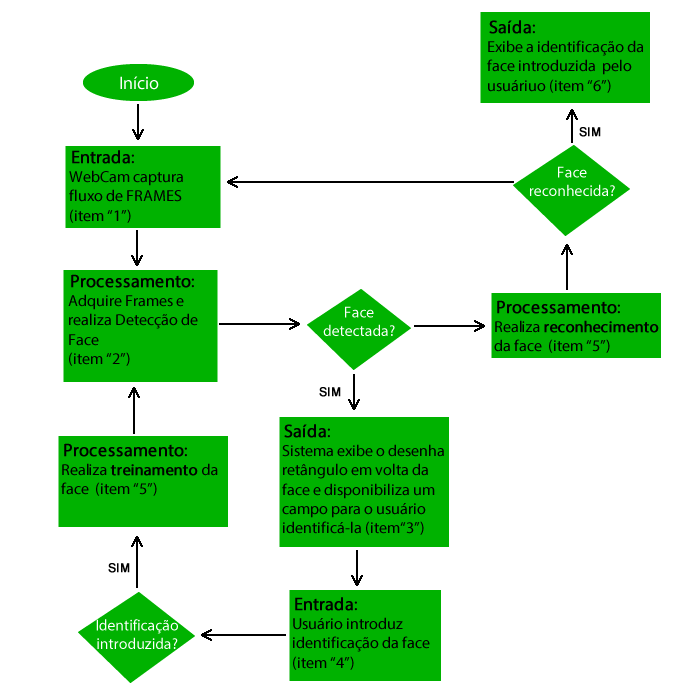
\includegraphics[width=.8\textwidth]{fluxo}
	\caption{Fluxograma representando os requisitos que devem ser atendidos.}
	\fonte{Elaborado pelo autor.}
	\label{fig:fluxoreq}
\end{figure}


\section{Diagrama de Pacotes}\label{sec:diagpacs}
Nesta seção, os pacotes criados implementação do sistema aqui proposto serão apresentadas em forma de diagrama de pacotes (UML). A \autoref{fig:SRFV_diagramaPacotes} ilustra tal diagrama:

\begin{figure}[h]
	\centering
	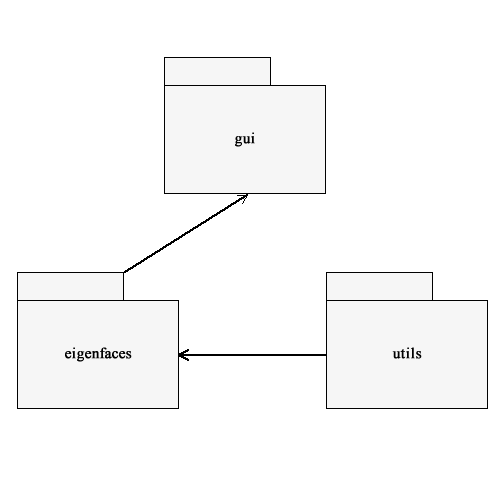
\includegraphics[width=.6\textwidth]{SRFV_diagramaPacotes}
	\caption{Diagrama de pacotes (UML) do sistema proposto.}
	\fonte{Elaborado pelo autor.}
	\label{fig:SRFV_diagramaPacotes}
\end{figure}

O pacote \textit{"gui"} possui classes responsáveis pela interface com o usuário e regras do sistema como controle de fluxo de quadros e execução de tarefas. O pacote \textit{"eigenfaces"} possui as classes responsáveis pelo execuçao do algoritmo ACP e a geração do espaço multidimensional de \textit{EigenFaces}. Por fim, o pacote de nome \textit{"utils"}, possui classes utilitárias resposáveis por manipular arquivos (carregar, salvar e deletar) e conversões de formatos de imagens. 

Na seção seguinte, cada pacote será descrito com seus respectivos diagramas de classe.

\section{Diagrama de Classes - Pacote \textit{\textbf{gui}}}\label{sec:diagclasses}
As classes do pacote \textbf{\textit{gui}} são representadas pelo diagrama (UML) na \autoref{figSRFV_diagramaClassse_gui}.

\begin{figure}[h]
	\centering
	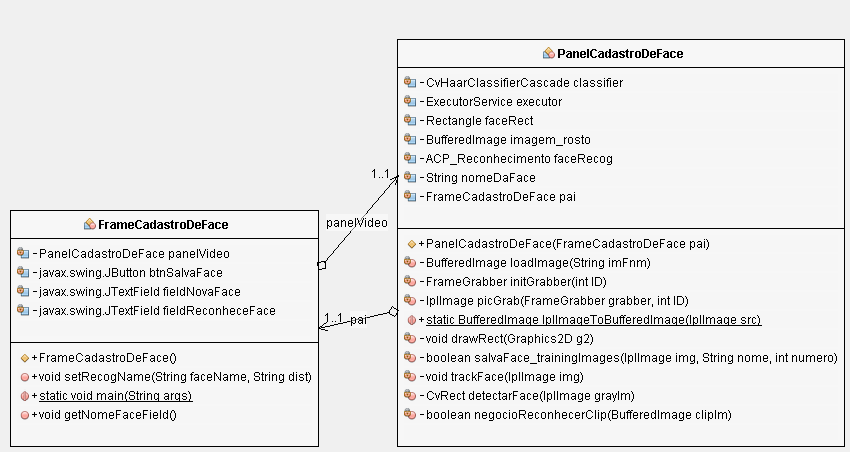
\includegraphics[width=.9\textwidth]{SRFV_diagramaClassse_gui}
	\caption{Diagrama de classes (UML) do pacote \textbf{\textit{gui}}.}
	\fonte{Elaborado pelo autor.}
	\label{figSRFV_diagramaClassse_gui}
\end{figure}

A classe \textbf{\textit{FrameCadastroDeFace}} é apenas uma janela com alguns componentes visuais, como um botão, um campo para entrada de informação e a tela para a visualizaçào do fluxo de quadros. A tela para visualização do fluxo é representada pela classe \textbf{\textit{PanelCadastroDeFace}}.

A classe \textbf{\textit{PanelCadastroDeFace}} também é responsávem pelo controle de frames e de execução de tarefas como a de deteção, treinamento e reconhecimento das faces. A seguir suas principais objetos e métodos são detalhados:

\begin{itemize}
	\item Objetos:
	\begin{itemize}
		\item \textbf{CvHaarClassifierCascade classifier}: classificadores pré treinados, assim como descritos na ????, para o processo de detecção da face;
		
		\item \textbf{ExecutorService executor:} este objeto é uma \textit{thread}. responsável por executar e controlar o processo de aquisiçao de quadros, deteção treinamento e reconecimento;
		
		\item \textbf{Rectangle faceRect:} objeto contendo a posição da face recem detectada em relação ao quadro retirado do vídeo;
		
		\item \textbf{BufferedImage imagem\_rosto:} objeto que salva um a imagem da face, caso detectada;
		
		\item \textbf{String nomeDaFace:} objeto que salva o nome da face detectada, informação esta que é entrada pelo usuário do sistema;
		
		\item \textbf{FrameCadastroDeFace pai:} objeto que referencia o seu parente de nível superior da classe \textbf{\textit{PanelCadastroDeFace}};
		
		\item \textbf{ACP\_Reconhecimento faceRecog:} objeto que instancia a classe responsável por executar o algoritmo de reconhecimento ACP, contido no pacote \textbf{\textit{eigenfaces}};
		
		\item \textbf{ACP\_Treinamento:} esta classe, contida no pacote \textbf{eigenfaces}, nao é instanciada como objeto porém é chamada de forma estática para produzir o espaço multidimensional a partir das imagens de treinamnto salvas em uma pasta especifica;
		
	\end{itemize}
	
	\item Métodos:
	\begin{itemize}
		\item \textbf{BufferedImage loadImage():} método que carrega imagem do sistema de arquivos para memória;
		
		\item \textbf{FrameGrabber initGrabber():} estabelece fluxo de quadros com a câmera;
		
		\item \textbf{IpiImage picGrab():} aquisita um quadro proveniente do fluxo de quadros;
		
		\item \textbf{void drawRect():} desenha um quadrado em volta do rosto aquisitado de acordo com as coordenadas do objeto \textbf{faceRect};
		
		\item \textbf{void salvaface\_treinamento()}: este método salva a face continda no objeto \textbf{imagem\_rosto} para futuro processo de treinamento;
		
		\item \textbf{void trackFace():} método chamado dentro da \textit{thread} ExecutorService executor que contém os processos e os controles de estado de detecção, treinamento e reconhecmento da face;
		
		\item \textbf{boolefan negocioReconhecerClip():} método chamado quando o sistema se encontra no estado de reconhecimento, onde o objeto \textbf{ACP\_Reconhecimento faceRegoc} é acionado;
	\end{itemize}
\end{itemize}

\section{Diagrama de Classes - Pacote \textit{\textbf{eigenfaces}}}\label{sec:diagclasses}
As classes do pacote \textbf{\textit{eigenfaces}} são representadas pelo diagrama (UML) da \autoref{figSRFV_diagramaClassse_eigenfaces} e descritas em seguida.

\begin{figure}[h]
	\centering
	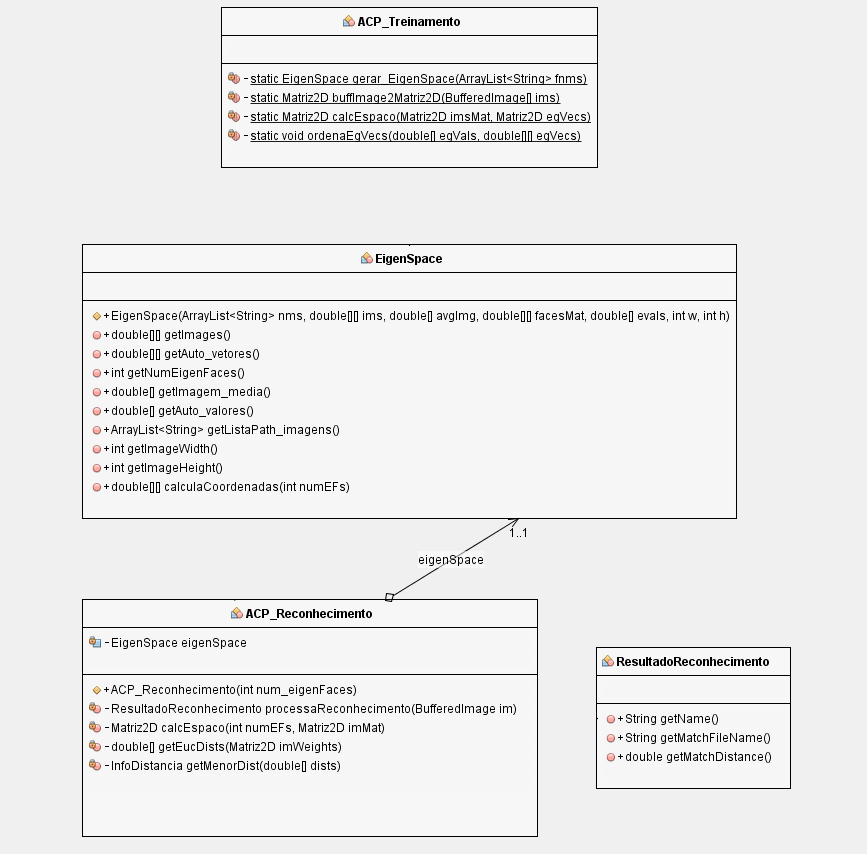
\includegraphics[width=1\textwidth]{SRFV_diagramaClassse_eigenfaces}
	\caption{Diagrama de classes (UML) do pacote \textbf{\textit{eigenfaces}}.}
	\fonte{Elaborado pelo autor.}
	\label{figSRFV_diagramaClassse_eigenfaces}
\end{figure}






\section{Diagrama de Classes - Pacote \textit{\textbf{utils}}}\label{sec:diagclasses}
As classes do pacote \textbf{\textit{utils}} são representadas pelo diagrama (UML) da \autoref{figSRFV_diagramaClassse_utils}. 

\begin{figure}[h]
	\centering
	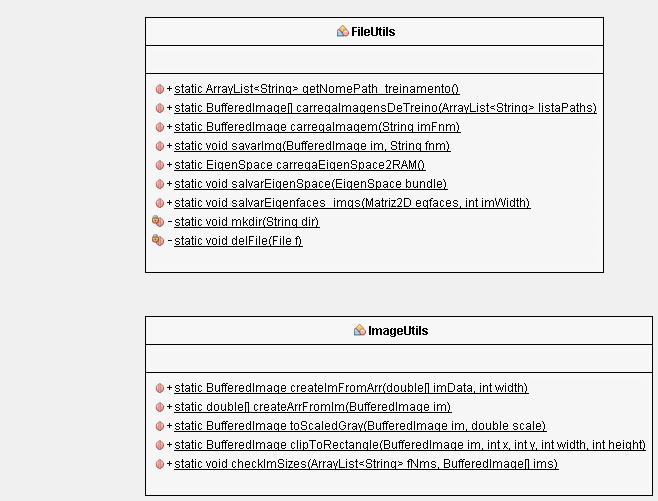
\includegraphics[width=.7\textwidth]{SRFV_diagramaClassse_utils}
	\caption{Diagrama de classes (UML) do pacote \textbf{\textit{utils}}.}
	\fonte{Elaborado pelo autor.}
	\label{figSRFV_diagramaClassse_utils}
\end{figure}












%\codigoPython
%\lstinputlisting[language=Python, label=coleta-script, caption=\textit{Script} coletar-hashtags.py]{src/coletar-hashtags.py}

%% !TeX encoding = UTF-8

\chapter{TESTES E ANÁLISE DOS RESULTADOS}\label{ch:resultados}

Este capítulo tem como finalidade apresentar os testes realizados através da manipulação das constantes definidas na \autoref{sec:consts}, seus resultados e posteriormente, a análise dos mesmos.

\section{Ambiente de Testes}\label{sec:ambtest}

Os testes foram realizados no local de trabalho do autor e os objetos de testes foram as faces dos funcionários do escritório do mesmo, dentro os quais a participação variava diariamente entre 6 a 10 participantes, incluindo o autor. Tomou-se cuidado para que as faces relacionadas fossem sempre as mesmas. Ou seja, a "face 1"\ seria a mesma face em todos os dias de treino.

Os equipamentos (\textit{hardwares}), descritos na \autoref{sub-hardw}, foram postos em um local de saída dos funcionários do escritóio, onde as condições luminosas eram sempre as mesmas.

A interface do sistema, como se pode ver na \autoref{screenshot-sys}, dispõe de uma máscara que indica o local em que a face deve ser posicionada corretamente em frente a câmera, e a câmera posicionada no mesmo local em todos os testes. A cada dia, caso o resultado de correspondência fosse considerada ruim (muito acima do valor mínimo \textit{MIN\_DIST}), ou caso o objeto de teste tenha se movido no momento do treino interrompendo o processo, a face poderia ser treinada novamente, o que acumularia as faces de treino do objeto de teste.

\begin{figure}[h]
	\centering
	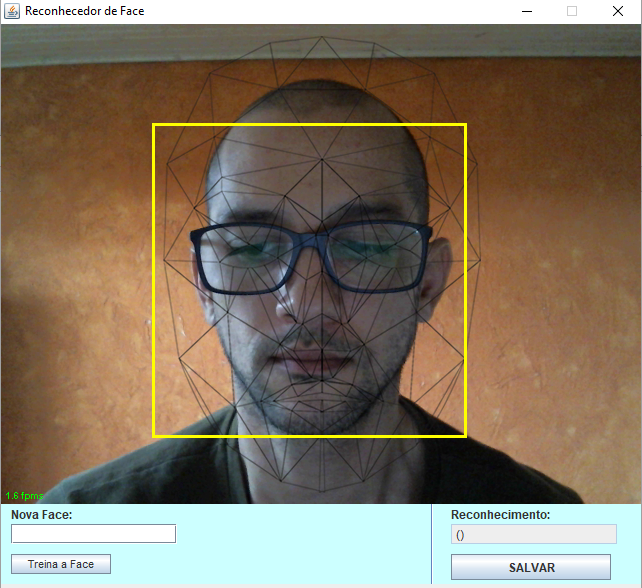
\includegraphics[width=1\textwidth]{screenshot-sys}
	\caption{Imagem do Sistema em Funcionamento.}
	\fonte{Elaborado pelo autor.}
	\label{screenshot-sys}
\end{figure}

Os usuários foram sujeitos ao teste sempre na mesma ordem. As faces dos objetos de testes foram expostas durante o tempo necessário para o sistema coletar a quantidade estabelecida pela constante \textit{NUM\_FACES\_TREINO}. O sistema foi configurado para faser cerca de 3 a 4 deteções por segundo.

Os testes documentados foram realizados em 5 (cinco) dias e divididos em três fases: duas fases de dois e uma fase de um dias. Para cada fase uma configuração distinta das constantes de controle contempladas na \autoref{sec:consts} foram definidas, as quais são detalhadas na seção seguinte.

Apresentam-se os resultados dos testes do sistema nas condições de cada fase em tabelas: uma para cada dia de teste. Todas apresentam as contagens das quantidades de reconhecimento realizadas por pessoa, bem como a nota média das distâncias correspodentes aos resultados de cada reconhecimento, tanto na falha quanto no sucesso, e a contagem de falsos positivos e falsos negativos.

A contagem dos resultados falsos positivos e falsos negativos foram feitos a olho nú e devidamente registrados pelo analista, comparando os resultados registrados pelo sistema no momento dos testes, como descreve a \autoref{sec:defsucregoc}.

\section{Testes e Resultados}\label{ch:testresult}

Esta sessão de testes, foi dividida em três fases: uma para cada configuração das constantes de controle. A finalidade de cada constante é contemplada na \autoref{sec:consts} e suas interações com o código descritas durante \autoref{sec:codigo}.


\subsection{Fase 1}\label{ch:testresultfaz1}
Para a primeira fase da \textit{sprint} testes, feita em dois dias, os valores das constantes de controle foram configuradas como define a lista abaixo.

\begin{itemize}	
	\item \textbf{NUM\_FACES\_TREINO = 2}
	\begin{itemize}	
		\item esta constante é resposável por controlar o número de faces a ser usado no treinamento, foi configurado para o valor 2 (dois) esperando-se manter um número reduzido de faces para treinamento, e consequentemente do tamanho do espaço multidimensional a ser gerado;
	\end{itemize}

	\item \textbf{NUM\_EF\_recog = 5}
	\begin{itemize}	
		\item esta constante é resposável por controlar o número de \textit{eigenfaces} ou auto-vetores a serem usadas no reconhecimento, foi configurado para o valor 5 (cinco), para se observar os resultados iniciais do experimento;
	\end{itemize}

	\item \textbf{MIN\_DIST = 0.433}
	\begin{itemize}	
		\item esta constante define se a distância encontrada na fase de reconhecimento pode ser considerada um resultado de sucesso ou falha, foi definida para o valor 0.433, para se observer os resultados iniciais.
	\end{itemize}
\end{itemize}

Estes valores iniciais foram definidos pelo desenvolvedor a partir de testes unitários não documentados em \textit{sprints} anteriores durante o desenvolvimento do sistema, onde os objetos de teste eram a face do próprio desenvolvedor, voluntários esporádicos ou imagens de faces.

Os resultados do primeiro dia de teste desta fase é descrito na \autoref{tab-res-fase1dia1}. Neste dia houveram 18 imagens de treinamento coletadas, com destaque para a "face 5", que por alguma razão, talvez sua pele muito branca e oleosa, refletia as luzes do ambiente dificultando o processo e apresentando maus resultados, e assim foi efetuada a coleta de mais imagens de treino deste usuário.

\begin{table}[h]
	\centering
	\caption{Resultado dos testes (Fase 1 - Primeiro dia) }
	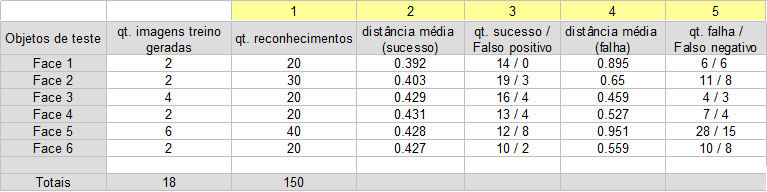
\includegraphics[width=1\textwidth]{tab-res-fase1dia1}
	\fonte{Elaborado pelo autor.}
	\label{tab-res-fase1dia1}
\end{table}

Os resultados do segundo dia de teste são apresentados na \autoref{tab-res-fase1dia2}. O esperado era que os usuários fossem reconhecidos com resultados parecidos. Observa-se que a "face 2 e 3"\ obtiveram maus resultados e tiveram que ser treinadas, possivelmente por faserem uso de maquiagem. A "face 5"\ continuou obtendo os maus resultados de anteriormente. Mais 4 faces foram adicionadas, acumulando um total de 22 imagens usadas para o treinamento.

\begin{table}[h]
	\centering
	\caption{Resultado dos testes (Fase 1 - Segundo dia) }
	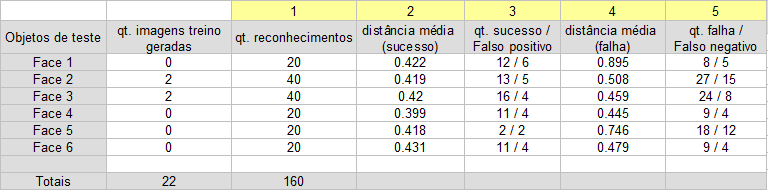
\includegraphics[width=1\textwidth]{tab-res-fase1dia2}
	\fonte{Elaborado pelo autor.}
	\label{tab-res-fase1dia2}
\end{table}



\subsection{Fase 2}\label{ch:testresultfaz2}
Para a segunda fase da \textit{sprint} testes, feita em dois dias, os valores das constantes de controle foram configuradas como define a lista abaixo. 

\begin{itemize}	
	\item \textbf{NUM\_FACES\_TREINO = 1}
	\begin{itemize}	
		\item esta constante é resposável por controlar o número de faces a ser usado no treinamento, foi configurado para o valor 1 (um) esperando-se reduzir ainda mais o espeço (em 50\%) para observar se diminui o numero de falsos positivos;
	\end{itemize}
	
	\item \textbf{NUM\_EF\_recog = 2}
	\begin{itemize}	
		\item esta constante foi configurado para o valor 2 (dois), para priozirar as \textit{eigenfaces} com mais probabilidade de ter atributos distintos entre as faces de treinamento, esperando-se observar um numero menor de falsos positivos
	\end{itemize}
	
	\item \textbf{MIN\_DIST = 0.55}
	\begin{itemize}	
		\item esta constante foi definida para o valor "0.55", esperando-se obervar uma melhor taxa de sucesso no reconhecimento.
	\end{itemize}
\end{itemize}

Os resultados do primeiro dia de teste desta fase é descrito na \autoref{tab-res-fase2dia1}. Neste dia coletou-se imagens de treino apenas de novos usuários, acumulando um total de 28 imagens de treino. 


\begin{table}[h]
	\centering
	\caption{Resultado dos testes (Fase 2 - Primeiro dia) }
	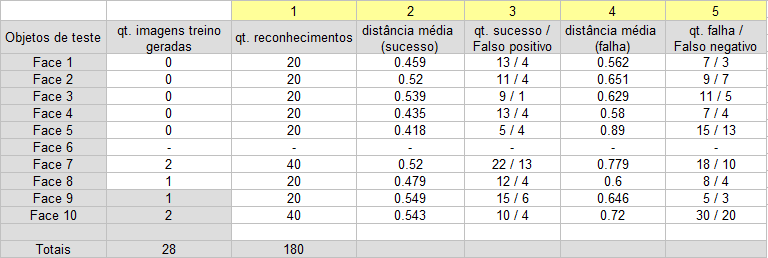
\includegraphics[width=1\textwidth]{tab-res-fase2dia1}
	\fonte{Elaborado pelo autor.}
	\label{tab-res-fase2dia1}
\end{table}


Os resultados do segundo dia de teste desta fase é descrito na \autoref{tab-res-fase2dia2}. Neste dia coletou-se uma imagem de cada usuário, acumulando um total de 35 imagens de treino. Foram feitos mais iterações de reconhecimento no usuário "face 5"\ pois este continuara a apresentar resultados maus (valores muito altos).


\begin{table}[h]
	\centering
	\caption{Resultado dos testes (Fase 2 - Segundo dia) }
	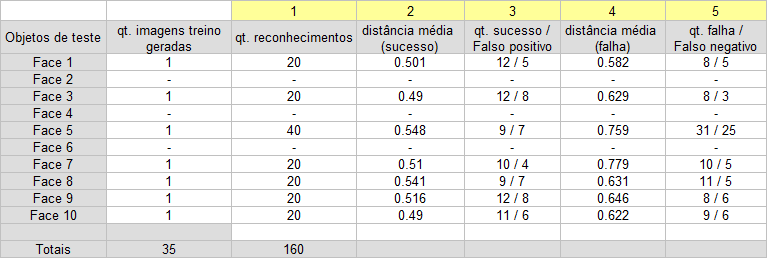
\includegraphics[width=1\textwidth]{tab-res-fase2dia2}
	\fonte{Elaborado pelo autor.}
	\label{tab-res-fase2dia2}
\end{table}



\subsection{Fase 3}\label{ch:testresultfaz3}
Para a terceira e últimas fase com apenas uma oportunidade para teste, as faces de treino foram deletadas para que se comece o teste com o espaço \textit{eigenspace} limpo/ Os valores das constantes de controle foram configuradas como define a lista abaixo.

\begin{itemize}	
	\item \textbf{NUM\_FACES\_TREINO = 7}
	\begin{itemize}	
		\item esta constante é resposável por controlar o número de faces a ser usado no treinamento, foi configurado para o valor 7 (sete) nesta fase, obter um valor maior de \textit{eigenfaces} geradas;
	\end{itemize}
	
	\item \textbf{NUM\_EF\_recog = 1}
	\begin{itemize}	
		\item esta constante foi configurado para o valor 1 (um), para descartar o máximo de \textit{eigenfaces} possível, afim de diminuir o número de falsos positivos;
	\end{itemize}
	
	\item \textbf{MIN\_DIST = 0.69}
	\begin{itemize}	
		\item esta constante foi definida para o valor "0.69", pois ao observar o teste anterior, analisou-se que em geral os resultados estavam piorando a medida que o número de imagens de treno aumentavam, e em muitos casos haviam muitos falsos negativos que poderiam ser confimação de sucesso.
	\end{itemize}
\end{itemize}

Os resultados desta fase de teste são apresentos na \autoref{tab-res-fase3}. Neste dia coletou-se 14 imagens de cada usuário, acumulando um total de 98 imagens de treino. Foram feitos mais iterações de reconhecimento para se ter uma melhor amostragem.

\begin{table}[h]
	\centering
	\caption{Resultado dos testes (Fase 3) }
	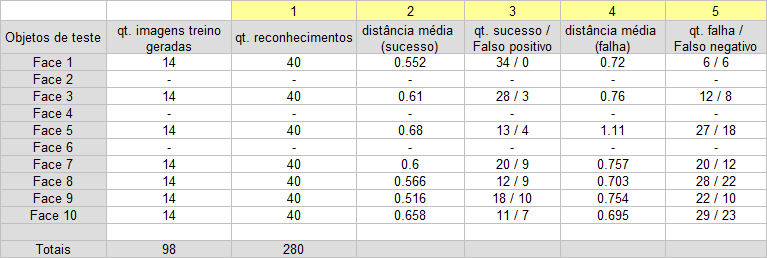
\includegraphics[width=1\textwidth]{tab-res-fase3}
	\fonte{Elaborado pelo autor.}
	\label{tab-res-fase3}
\end{table}





\section{Análise dos Resultados}\label{ch:analresult}

Ao decorrer dos testes e se analisar os resultados iniciais, pode-se perceber logo de início que a técnica é extremamente sensível a luzes/sombras, poses e expressões. Algo que pode variar muito a reflexão da luz na face do usuário é a cor da pele, oleosidade, maquiagem e acessórios como boné ou chapéu. Um mínimo movimento no momento da coleta das imagens de treino pode causar uma grande diferença no resultado.

Como se pode verificar na \autoref{taxarecogfases}, na primeira fase foram feitos 310 reconhecimentos sendo que 149 foram considerados pelo sistema como sucesso. Destes, apenas 103 foram de fato equivalentes, apresentando a taxa real de reconhecimento com \textit{33.22\%} de sucesso. Dos reconhecimentos considerados como falha somaram o total de 161, dos quais 92 eram falsos negativos, pois se tratava de uma real equivalência. Sendo assim, 55\% das falhas deveriam ser reconhecimento de sucesso. 

\begin{table}[h]
	\centering
	\caption{Taxas de sucesso reais dos reconhecimentos nas fases de teste.}
	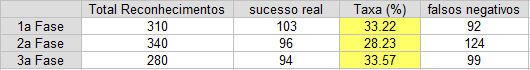
\includegraphics[width=.8\textwidth]{taxarecogfases}
	\fonte{Elaborado pelo autor.}
	\label{taxarecogfases}
\end{table}

Observou-se, que dependendo da face e suas condições, as médias das distâncias euclidianas poderiam variar forma imprevisível. Algumas faces tinham bons resultados de reconhecimento enquanto outras os apresentavam péssimos, em relação à constante \textit{MIN\_DIST}. O grande número de falsos negativos apresentados incentivaram a reconfiguração da constante \textit{MIN\_DIST} para um valor maior, \textit{NUM\_FACES\_TREINO} foi reduzido para que o espaço não sofresse muita adição de tamanho, \textit{NUM\_EF} foi reduzido para priorizar \textit{eigenfaces}, e apenas treinos de novas faces foram realizadas, esperando-se que os resultados de reconhecimento melhorassem ou se mantivessem.


Na segunda fase foram feitos 340 reconhecimentos sendo que 185 foram considerados pelo sistema como sucesso. Destes, 96 foram de fato equivalentes. Sendo assim, apresentando a taxa real de reconhecimento de \textit{28.3\%} de sucesso. Dos reconhecimentos considerados como falha, que somaram o total de 195, 124 se tratavam de uma real equivalência. Sendo assim 63.5\% das falhas deveriam ser reconhecimento de sucesso.

Observa-se que,os resultados da segunda fase foram piores que o da anterior, porém as contagens de falsos positivos e negativos ainda se apresentavam elevadas. Reconfigurou-se então as variáveis como conta na \autoref{ch:testresultfaz3} levando em conta lógica de que se um maior número de possível da coleta de imagens de uma face para o treino, combinado com o descarte de auto-vetores por auto-valores, "filtraria"\ melhor as caracteristicas da face e suas variáveis (sombras e reflexoes, movimentos, feiçoes ou enquadramento da face) melhor registradas. A constante \textit{MIN\_DIST} também sofreu adição de valores para que se diminuíse ainda mais os falsos negativos que poderiam ser reconhecimentos de sucesso, com cautela para não provocar resultados falsos positivos.

Segundo os resultados da terceira fase, foram feitos 280 reconhecimentos sendo que 136 foram considerados pelo sistema como sucesso. Destes, apenas 94 foram de fato equivalentes, apresentando a taxa real de reconhecimento com \textit{33.57\%} de sucesso. Dos reconhecimentos considerados como falha (total de 144), 99 se tratava de uma real equivalência. Sendo assim cerca de 50\% das falhas deveriam ser reconhecimento de sucesso.

Observou-se então uma melhora considerável nos resultados, levando em conta que o espaço de eigenfaces era muito maior relacionada às duas primeiras fases, porém ainda é um valor que não apresenta precisão e confiabilidade. 

Não obstante, desconsiderando a constante \textit{MIN\_DIST} e analisando apenas a contagem de resultados de sucesso (com falsos positivos já subtraídos) somandos com a contagem dos falsos negativos, verificamos que na maioria das vezes o algoritmo \textit{Eigenfaces} conseguiu equivalência de sucesso, como mostram os resultados dos testes apresentados.


\begin{figure}[h]
	\centering
	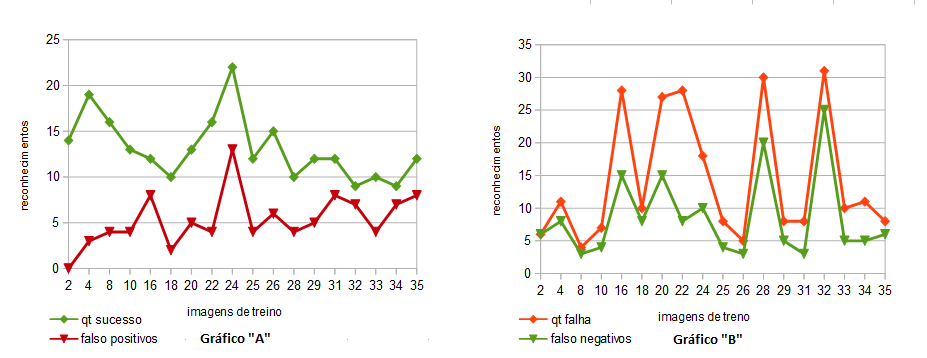
\includegraphics[width=1.1\textwidth]{grafab-fase12}
	\caption{\textbf{Gráfico "A"}: Reconhecimentos de sucesso (eixo Y) por quantidade de imagens usadas para o treino (eixo X). \textbf{Gráfico "B"}: Falhas no reconhecimentos (eixo Y) por quantidade de imagens usadas para o treino (eixo X). Referentes as fases de teste "1" e "2".}
	\fonte{Elaborado pelo autor.}
	\label{grafab-fase12}
\end{figure}

\begin{figure}[h]
	\centering
	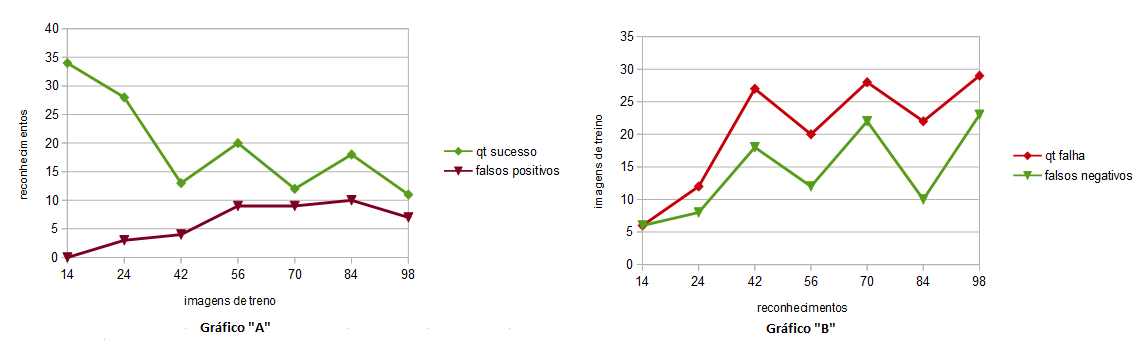
\includegraphics[width=1.1\textwidth]{grafab-fase3}
	\caption{\textbf{Gráfico "A"}: Reconhecimentos de sucesso (eixo Y) por quantidade de imagens usadas para o treino (eixo X). \textbf{Gráfico "B"}: Falhas no reconhecimentos (eixo Y) por quantidade de imagens usadas para o treino (eixo X). Referentes as fases de teste "3".}
	\fonte{Elaborado pelo autor.}
	\label{grafab-fase3}
\end{figure}


As \autoref{grafab-fase12} e \autoref{grafab-fase3} apresentam dois gráficos: os gráficos "\textit{A}" são às contagens de reconhecimentos de sucesso (eixo \textit{Y}) a medida em que a quantidade de imagens de treino cresce (eixo \textit{X}), e os gráficos "\textit{B}", são as contagens de falhas de reconhecimento a medida em que as imagens de treinamento crescem. A \autoref{grafab-fase12} se refere aos resultados da fase "1"\ e "2", e a \autoref{grafab-fase3} é referente à fase "3". Foram divididos desta forma pelo fato de quem o espaço foi reiniciado no terceiro dia, como descreve a \autoref{ch:testresultfaz3}. 

Analisando-os, observa-se que nos dois gráficos "A", as linhas de quantidade de sucesso e falsos positivos tendem a se encontram enquanto que nos gráficos "B"\ das duas figuras, o contrário acontece: as linhas de quantidade de falhas e de falsos negativos tendem a se afastar, apesar de não estar tão evidenciado no gráfico "B"\ da \autoref{grafab-fase12}, podendo-se concluir que à medida em que o espaço multidimensional de \textit{eigenfaces} (\textit{eigenspace}) cresce, o método ACP apresenta distâncias falsas e verdadeiras similares, imprecisando seu veridito final.














%GRAFICOSSS PARA

%\begin{grafico}[h]
%	\centering
%	\fbox{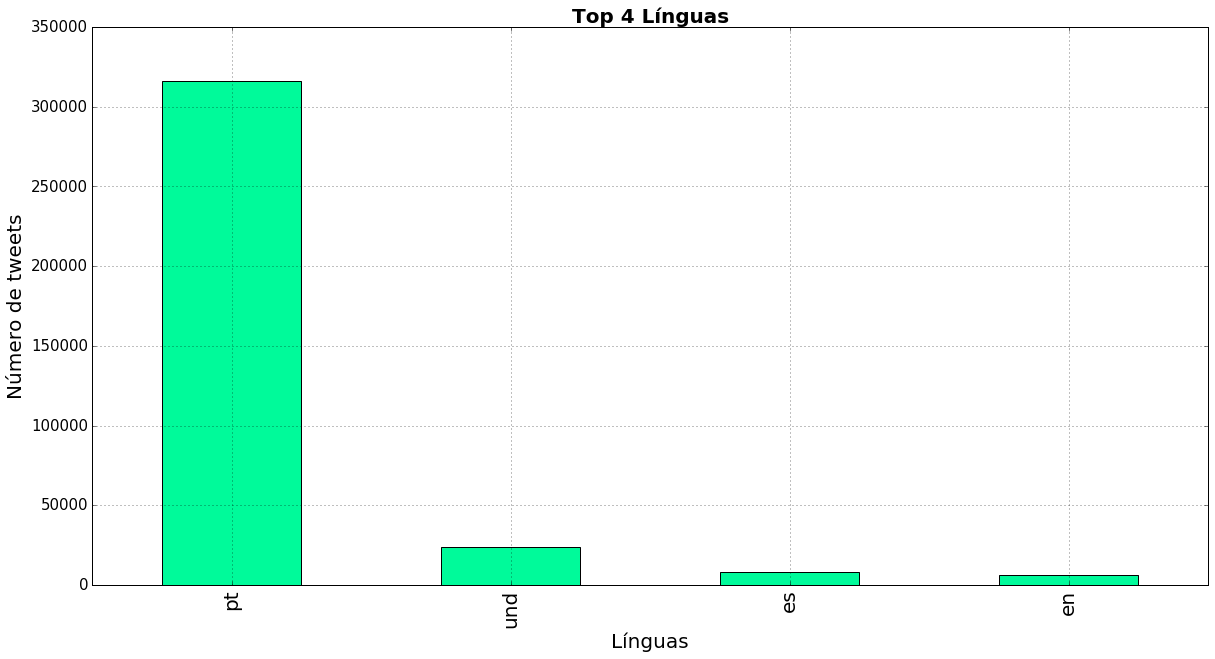
\includegraphics[width=1\textwidth]{linguas}}
%	\caption{Idiomas que mais realizaram \textit{tweets}}
%	\fonte{Elaborado pelo autor}
%	\label{lingua}
%\end{grafico}










%% !TeX encoding = UTF-8

\chapter{CONCLUSÕES E SUGESTÕES PARA FUTUROS TRABALHOS}\label{ch:conclusao}
\section{CONCLUSÕES} 
O uso das bibliotecas que Python oferece para a mineração de dados...

- Resgatar o objetivo

- Comentar as ferramentas estudadas

- Comentar as ferramentas utilizadas

- Breve resumo dos resultados

- Pontos positivos e negativos (O fato de não ter o perfil real)


\section{SUGESTÕES PARA FUTUROS TRABALHOS}

%
%7.2
%Pensar em outra API (Aplicação para previsão de resultados) ou rede social, baseando-se numa pergunta específica

%\bookmarksetup{startatroot}

%==============================================================================
% ELEMENTOS PÓS-TEXTUAIS
%==============================================================================
\postextual

% ------------------------------------ %
% Arquivo de bibliografias do trabalho %
% ------------------------------------ %
\label{biblio}\bibliography{Configuracoes/citacoes}

{\ }\label{fimBiblio}

\pagebreak
\ 


%==============================================================================
% APÊNDICES
%==============================================================================

%\begin{apendicesenv}% Apêndices: inserir se necessário
%\partapendices
%  \input{Extras/apendice1}
%  \input{Extras/apendice2}
%\end{apendicesenv}

%\begin{anexosenv}% Anexos: inserir se necessário
%\partanexos
% \input{Extras/anexo1}
% \input{Extras/anexo2}
% \input{Extras/anexo3}
%\end{anexosenv}

\printindex		% Indice Remissivo


\end{document}
